\documentclass[final,3p,times,12pt]{article}
\usepackage[utf8]{inputenc}
\usepackage{graphicx, float} 
\graphicspath{{images/}}
\usepackage{amsmath, amssymb, amsthm}
\usepackage{subcaption}
\usepackage[title,titletoc]{appendix}
\usepackage[utf8]{inputenc} % Required for inputting international characters
\usepackage[T1]{fontenc} % Output font encoding for international characters
\usepackage{graphicx}
\usepackage{enumitem}
\usepackage{longtable}
\usepackage{stmaryrd}
%\usepackage{mathpazo} % Palatino font
\usepackage[colorlinks=true, linkcolor=black, citecolor=black, urlcolor=black]{hyperref}
\usepackage{array}
\usepackage[svgnames]{xcolor}
% Define the dark green color
\definecolor{darkgreen}{rgb}{0.0, 0.5, 0.0} % Adjust RGB values as needed
% Setting margin sizes
\usepackage[letterpaper, top=1.0in, bottom=1.0in, left=1.0in, right=1.0in, heightrounded]{geometry}
% Line height
\renewcommand{\baselinestretch}{1.15} % linespacing
% Parskip and Parindent (sets the space between paragraphs)
\setlength{\parskip}{0.8em}
\usepackage{tocloft}
\setlength{\cftbeforesecskip}{5pt}
\setlength{\cftbeforesubsecskip}{5pt}
\setlength{\cftbeforesubsubsecskip}{5pt}
\usepackage{caption}  % For captions under figures
\bibliographystyle{ieeetr}
\usepackage{listings}
\usepackage{color}
\usepackage{booktabs}


% Define the style for Python code
\lstdefinestyle{pythoncode}{
  language=Python,
  basicstyle=\scriptsize,
  keywordstyle=\color{blue},
  commentstyle=\color{darkgreen},
  stringstyle=\color{red},
  showstringspaces=false,
  identifierstyle=\color{black},
  procnamekeys={def,class},
  frame=single, % adds a frame around the code
  rulecolor=\color{black}, % if not set, the frame-color may be changed on line-breaks within not-black text
  breaklines=true, % sets automatic line breaking
  captionpos=b, % sets the caption-position to bottom
  numbers=left, % where to put the line-numbers
  numberstyle=\tiny\color{black}, % the style that is used for the line-numbers
  numbersep=10pt, % how far the line-numbers are from the code
  tabsize=4, % sets default tabsize to 2 spaces
}
\lstset{style=pythoncode}

\begin{document}

\begin{titlepage}
    \centering
    \vspace*{2cm}
    
    {\Large \textbf{COMP0078}}\\[1cm] % Module Code
    {\Huge \textbf{Supervised Learning Coursework 1}}\\[1cm] % Title
    
    \vspace{1cm}
    
    {\Large November 2024}\\[1.5cm] % Date
    
    % Optional additional information, like your name or university
    {\Large University College London} % Replace with your university name if applicable
    
    \vfill
    
    % Optional logo placement (if desired)
    % \includegraphics[width=0.3\textwidth]{path_to_your_logo.png}
    
    \vspace{2cm}
    
\end{titlepage}
\newpage

\tableofcontents
\newpage


\section{Part 1}

\subsection{Linear Regression}

\begin{enumerate} % This is Linear regressison
    \item Fitting polynomials of order $k \in \{1, 2, 3, 4\}$ to 4 data points. % This is question 1
    \begin{enumerate} 
        \item The plot for the polynomial bases fit to the four data points is shown in Figure \ref{fig:question_1a}:

        \begin{figure}[H]
            \centering
            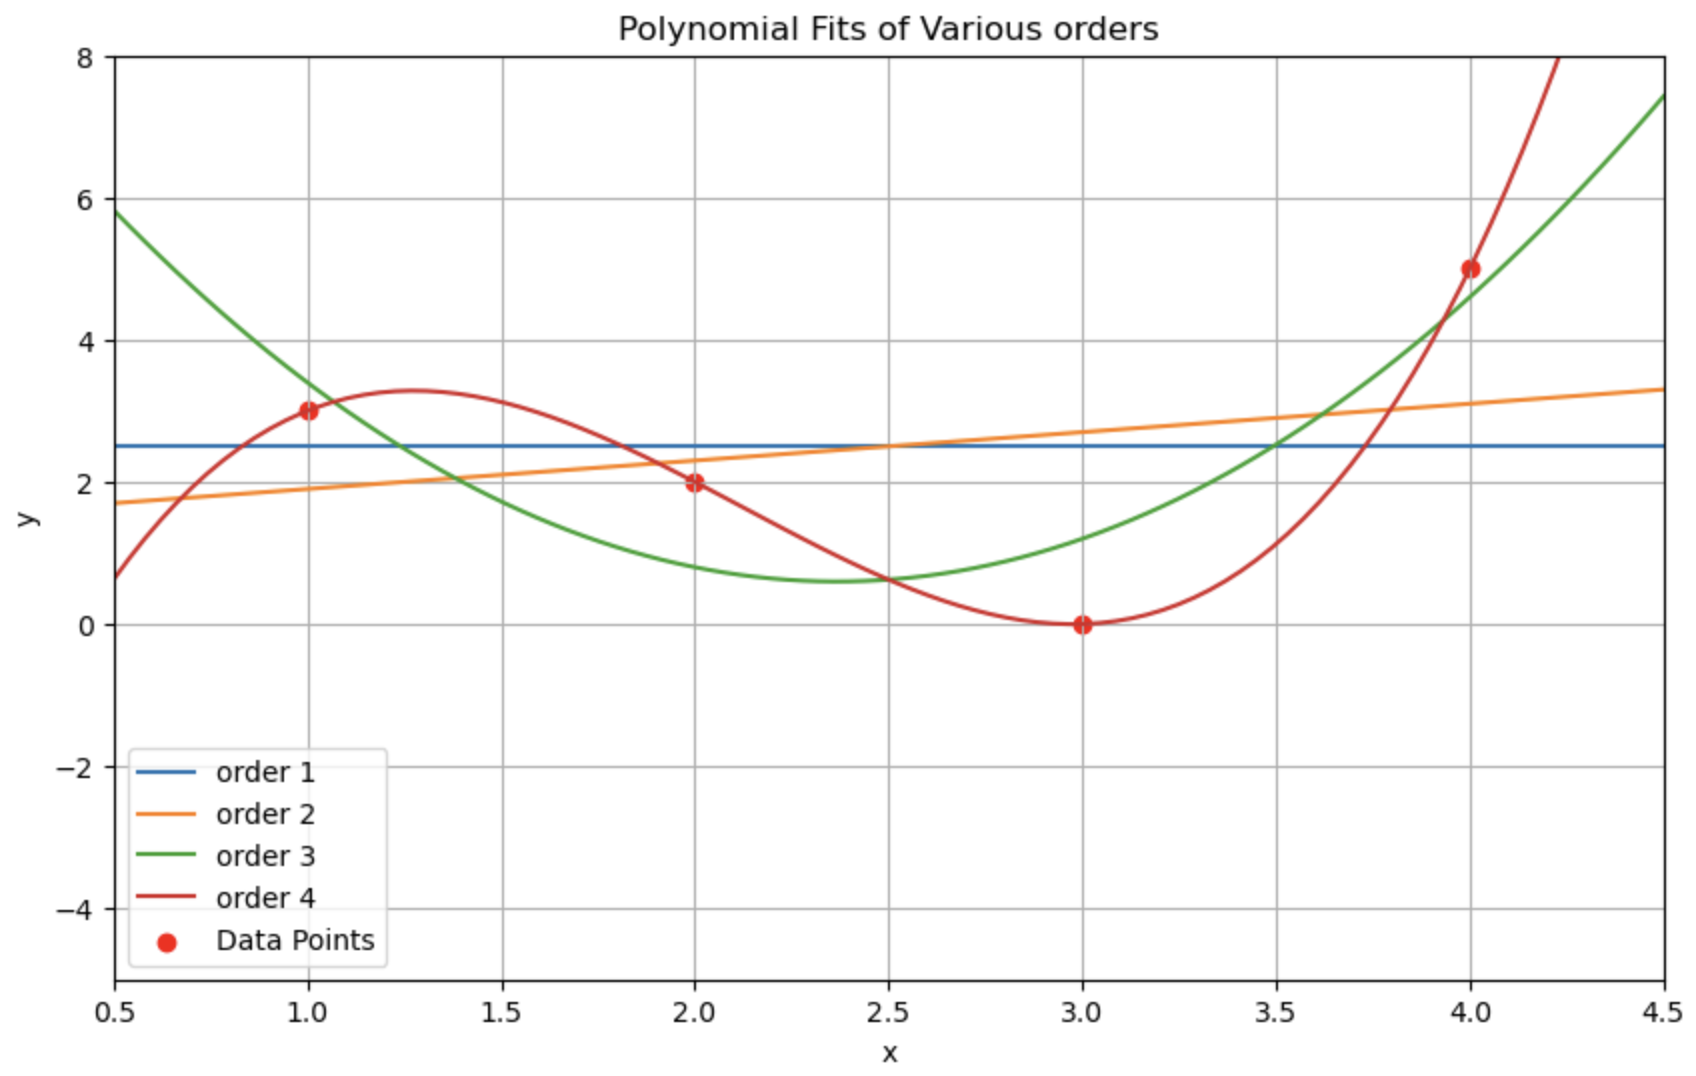
\includegraphics[width=0.7\textwidth]{images/question_1a.png}
            \caption{Figure showing the plots of the fitted polynomials with orders $\in \{1, 2, 3, 4\}$}
            \label{fig:question_1a}
        \end{figure}

        For the rest of Part I and in the code, we use the term "order" to reference the dimensions of the polynomial bases. Figure \ref{fig:question_1a} is similar to the one given in the question as expected. 

        \item  The equations corresponding to the curves fitted for $k = 1, 2, 3$ are given in Table \ref{tab:polynomial_mse}:


        \item The Mean Square Error (MSE) for each fitted curved is also given in Table \ref{tab:polynomial_mse}. We see that the MSE decreases as the order increases. 

        \begin{table}[H]
        \centering
        \begin{tabular}{|c|l|c|}
        \hline
        \textbf{Polynomial Order} & \textbf{Equation} & \textbf{MSE} \\ \hline
        1 & \(y = 2.50x^0\) & \(3.25 \times 10^0\) \\ \hline
        2 & \(y = 1.50x^0 + 0.40x^1\) & \(3.05 \times 10^0\) \\ \hline
        3 & \(y = 9.00x^0 - 7.10x^1 + 1.50x^2\) & \(8.00 \times 10^{-1}\) \\ \hline
        4 & \(y = -5.00x^0 + 15.17x^1 - 8.50x^2 + 1.33x^3\) & \(5.82 \times 10^{-24}\) \\ \hline
        \end{tabular}
        \caption{Table showing the polynomial equations and their MSE values}
        \label{tab:polynomial_mse}
        \end{table}
    \end{enumerate}
    
    \item Illustrating the phenomena of overfitting.  % This is question 2
    \begin{enumerate}
        \item Generating data and fitting polynomial bases 
        \begin{enumerate}
            \item The plot the function $sin^2(2\pi x)$ in the range $0 \leq x \leq 1$ with the points of the above data set superimposed is shown in Figure \ref{fig:question_2ai}:

            \begin{figure}[H]
                \centering
                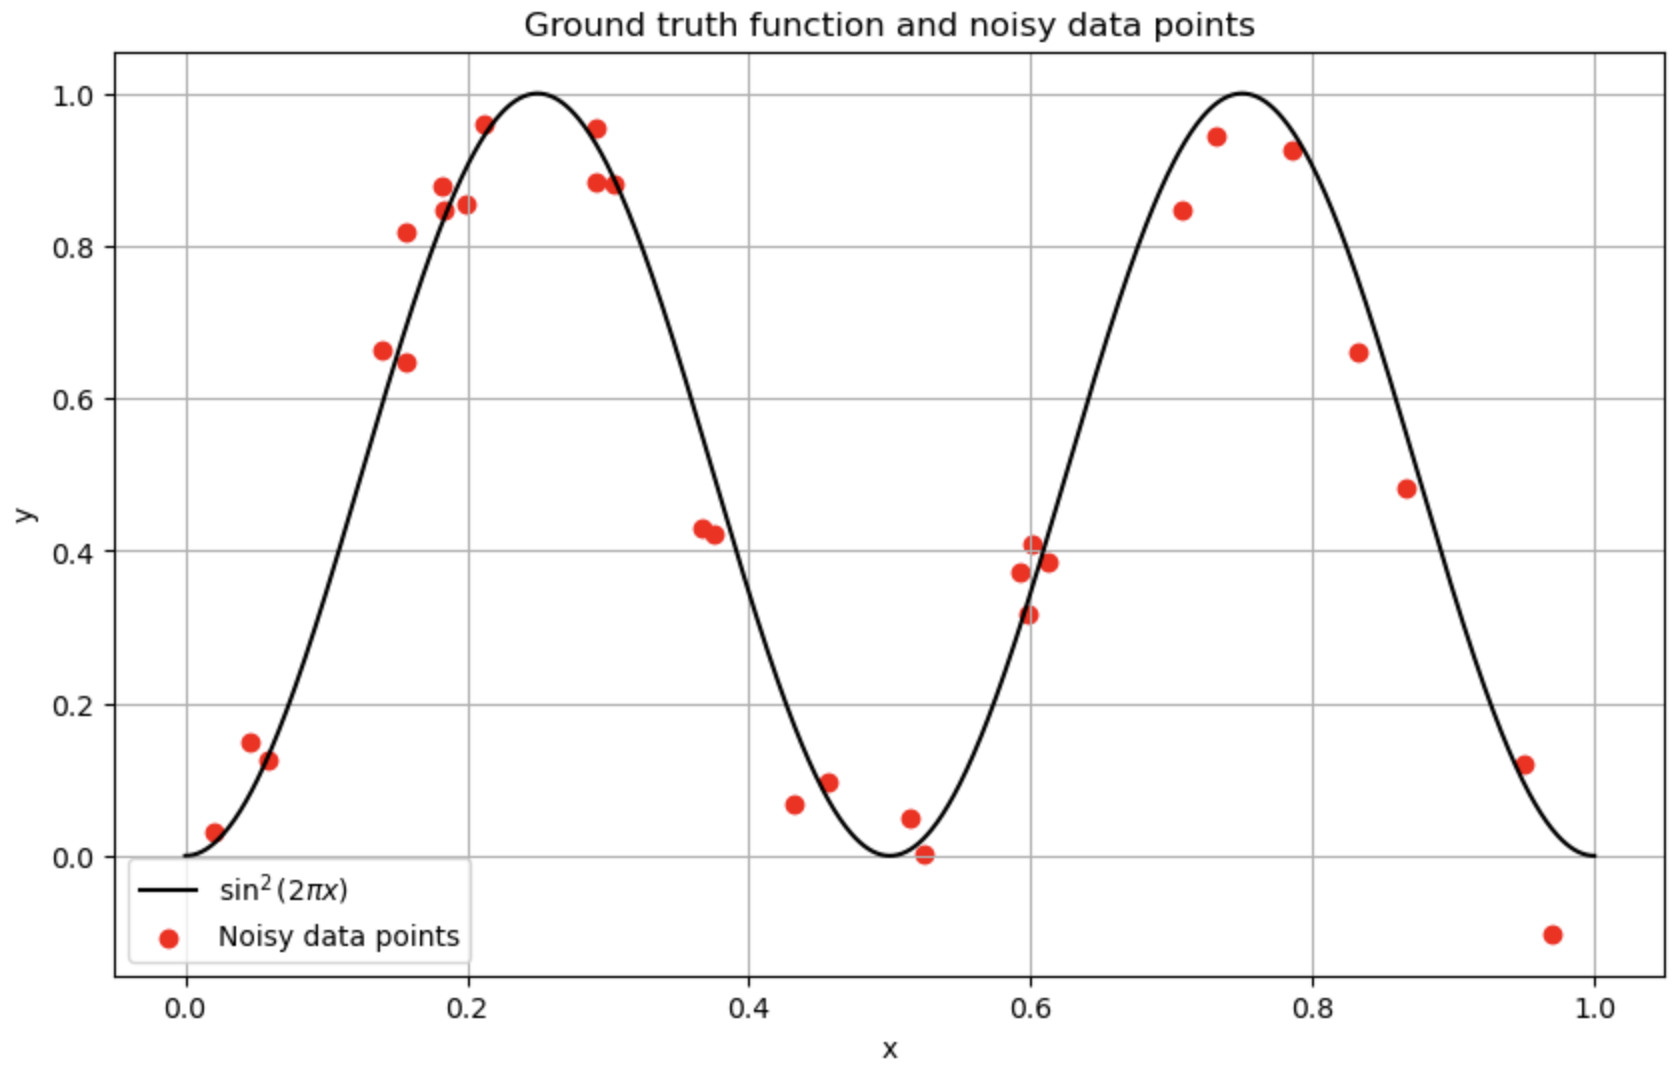
\includegraphics[width=0.7\textwidth]{images/question_2ai.png}
                \caption{Figure showing the function plotted on top of the generated data}
                \label{fig:question_2ai}
            \end{figure}
            Figure \ref{fig:question_2ai} resembles the provided plot as expected. 
            
            \item The plot showing the fit of the data set with polynomial bases of dimension $k = 2, 5, 10, 14, 18$ is given in Figure \ref{fig:question_2aii}:

            \begin{figure}[H]
                \centering
                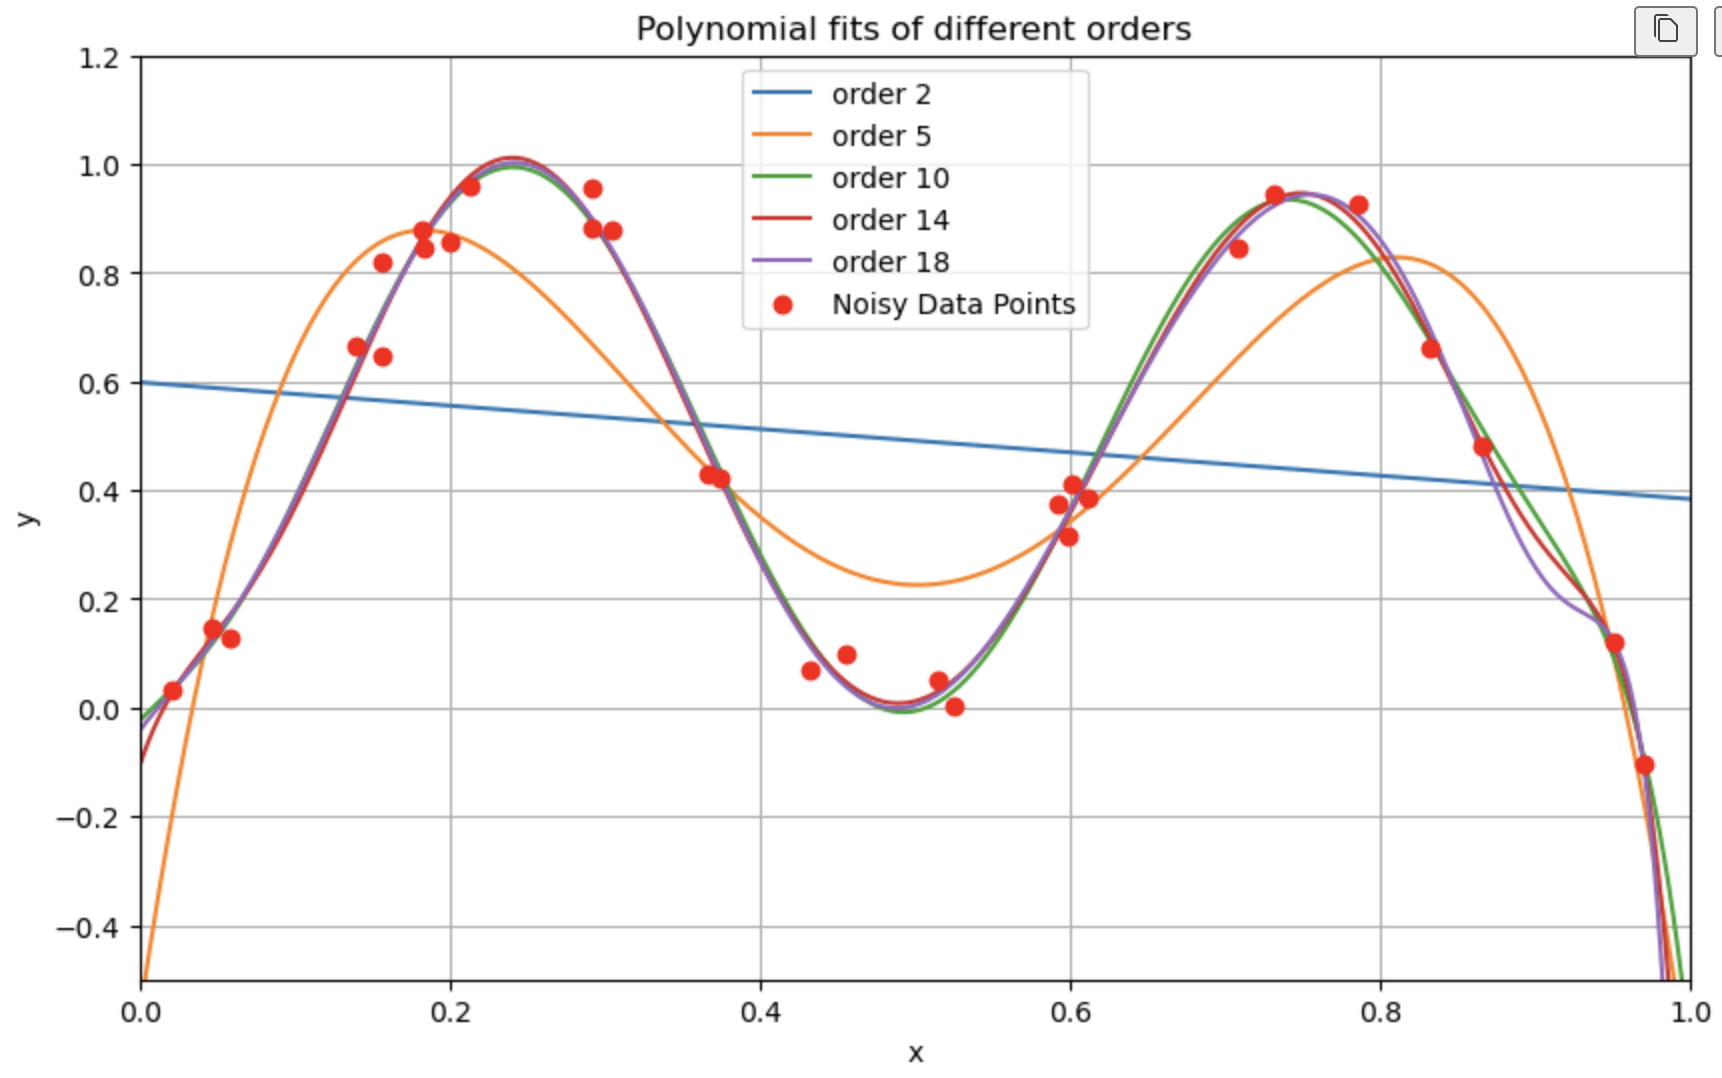
\includegraphics[width=0.7\textwidth]{images/question_2aii.png}
                \caption{Figure showing the fit of the data set with the different polynomials}
                \label{fig:question_2aii}
            \end{figure}
        \end{enumerate}

        \item The plot the natural log of the training error versus the polynomial dimension is given in Figure \ref{fig:question_2b}

        \begin{figure}[H]
            \centering
            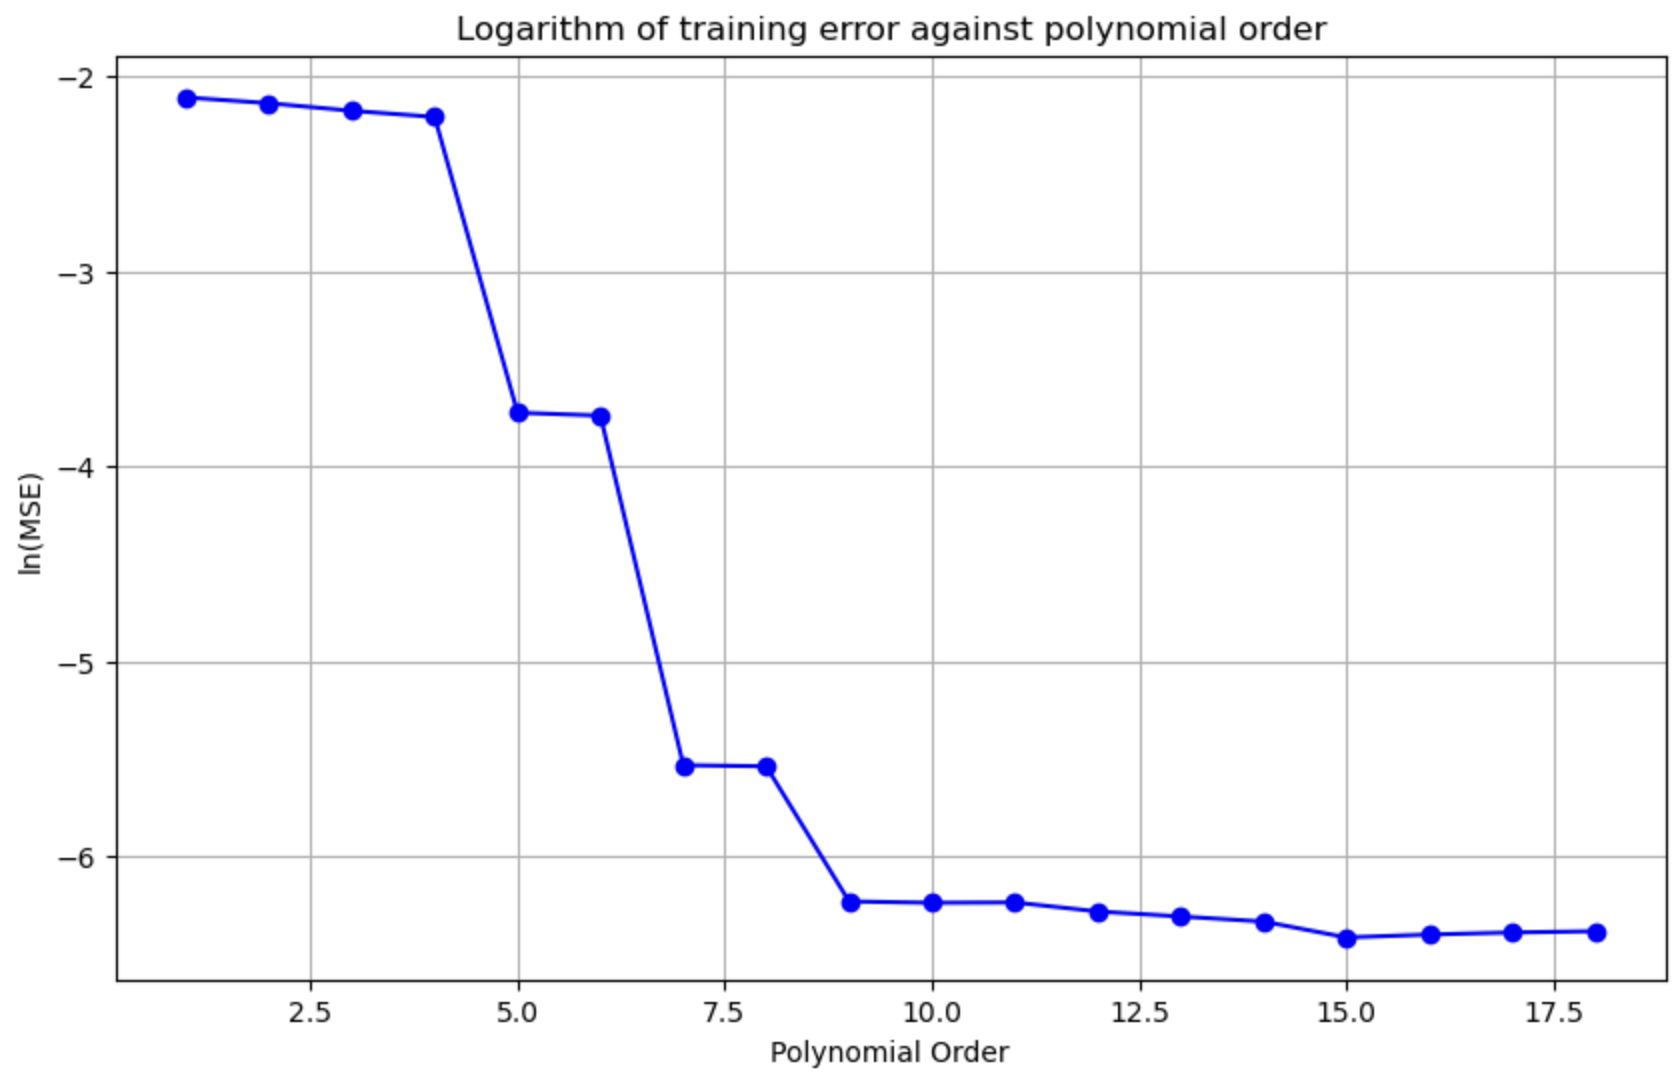
\includegraphics[width=0.7\textwidth]{images/question_2b.png}
            \caption{Figure showing the plot the natural log of the training error versus the polynomial dimension}
            \label{fig:question_2b}
        \end{figure}
        This is a decreasing function, as required. 

        \item  The plot the natural log of the test error versus the polynomial dimension is shown in Figure \ref{fig:question_2c}:

         \begin{figure}[H]
            \centering
            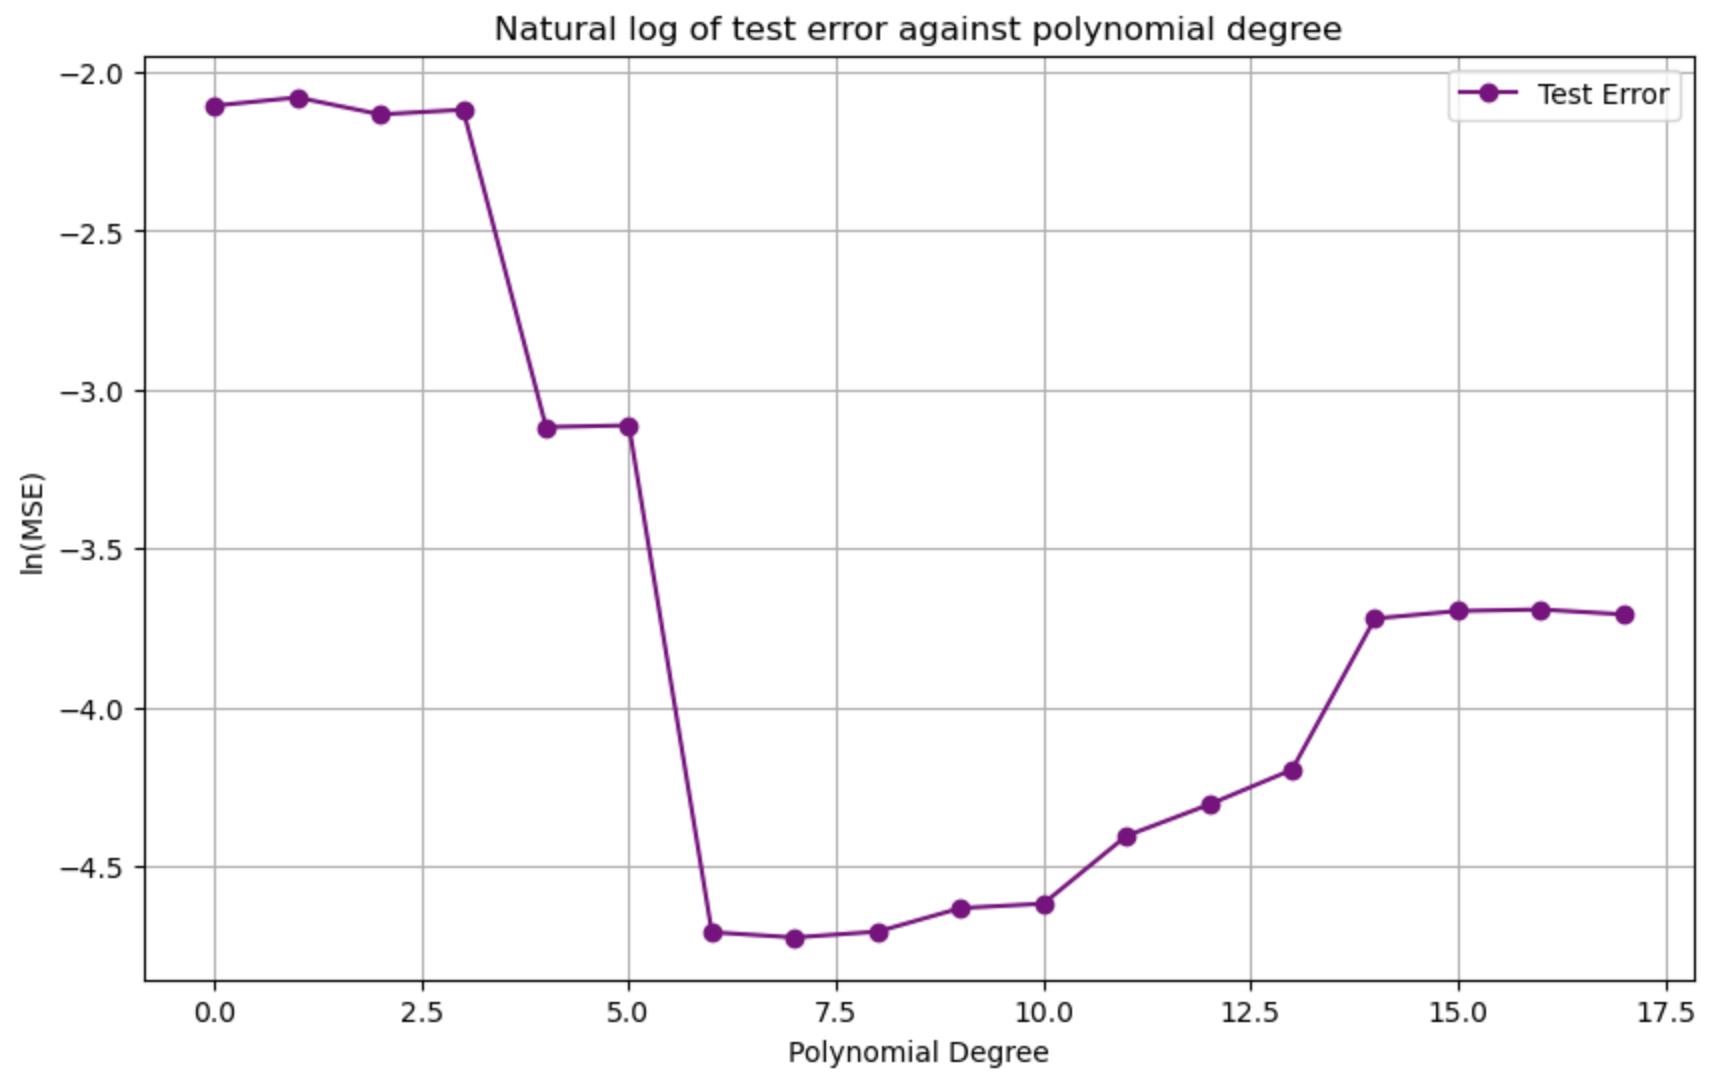
\includegraphics[width=0.7\textwidth]{images/question_2c.png}
            \caption{Figure showing the plot the natural log of the test error versus the polynomial dimension}
            \label{fig:question_2c}
        \end{figure}
        In the figure above, we can see the overfitting in the increase of test error starting at $k=6$.

        \item The plot showing the average result for the training and test errors over 100 runs is given in Figure \ref{fig:question_2d}:
         \begin{figure}[H]
            \centering
            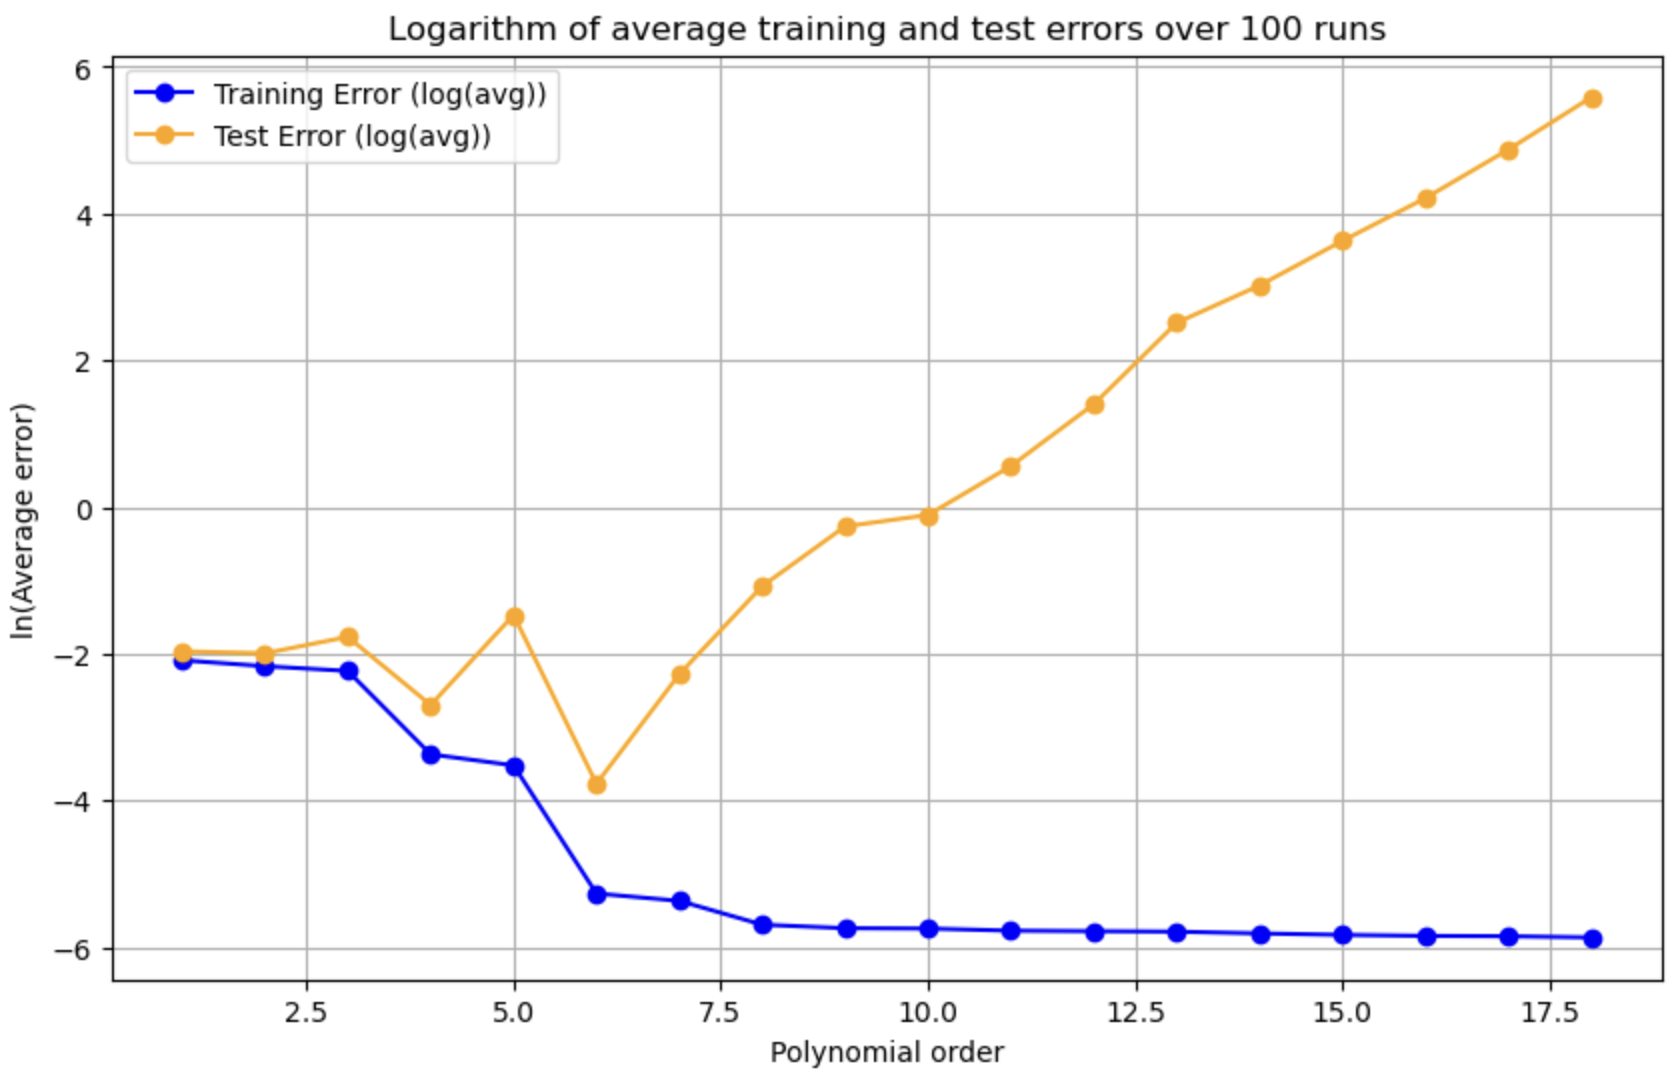
\includegraphics[width=0.7\textwidth]{images/question_2d.png}
            \caption{Figure showing the plot showing the average result for the training and test errors over 100 runs}
            \label{fig:question_2d}
        \end{figure}
    \end{enumerate}

    \item In this question, we repeating questions 2b to 2d using a sine basis instead of a polynomial one. The plot of the training error against the order of the sine basis is shown in Figure \ref{fig:question_3b}, the test error against the order of the sine basis in Figure \ref{fig:question_3c} and the average train and test error over 100 runs in Figure \ref{fig:question_3d}:
    
    \begin{figure}[H]
        \centering
        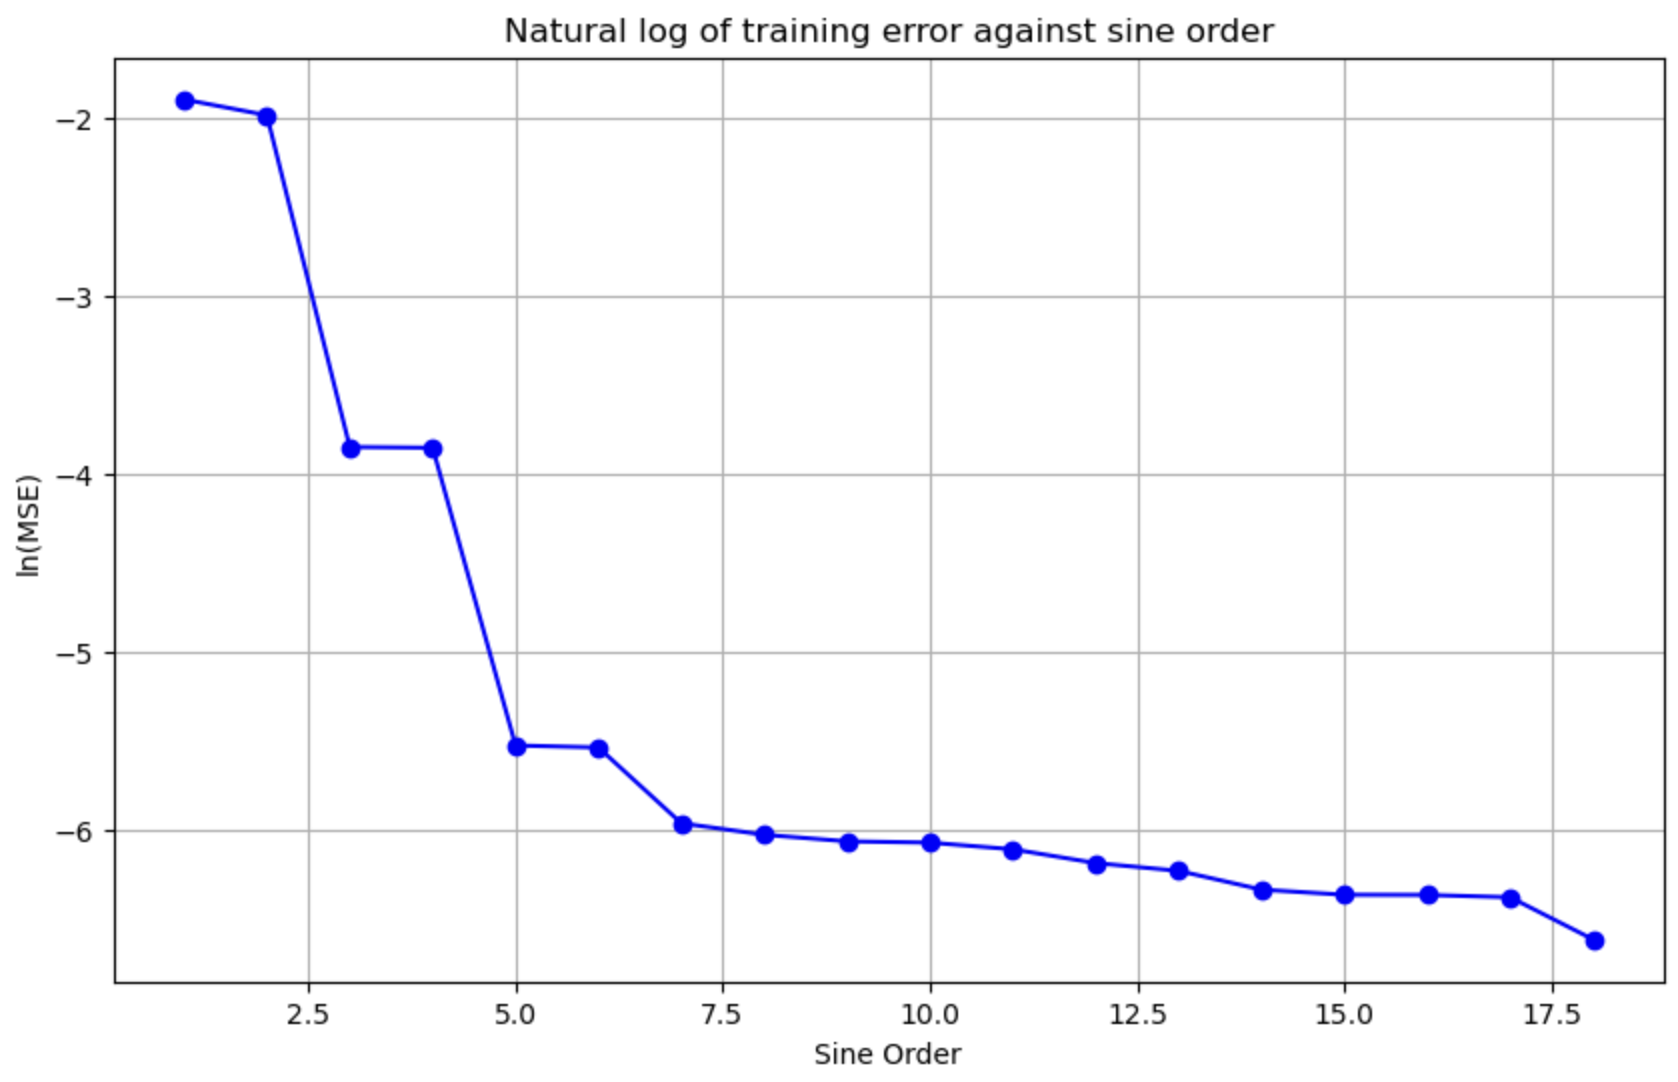
\includegraphics[width=0.7\textwidth]{images/question_3b.png}
        \caption{Figure showing the plot showing the training error against the order of the sine basis}
        \label{fig:question_3b}
    \end{figure}

    \begin{figure}[H]
        \centering
        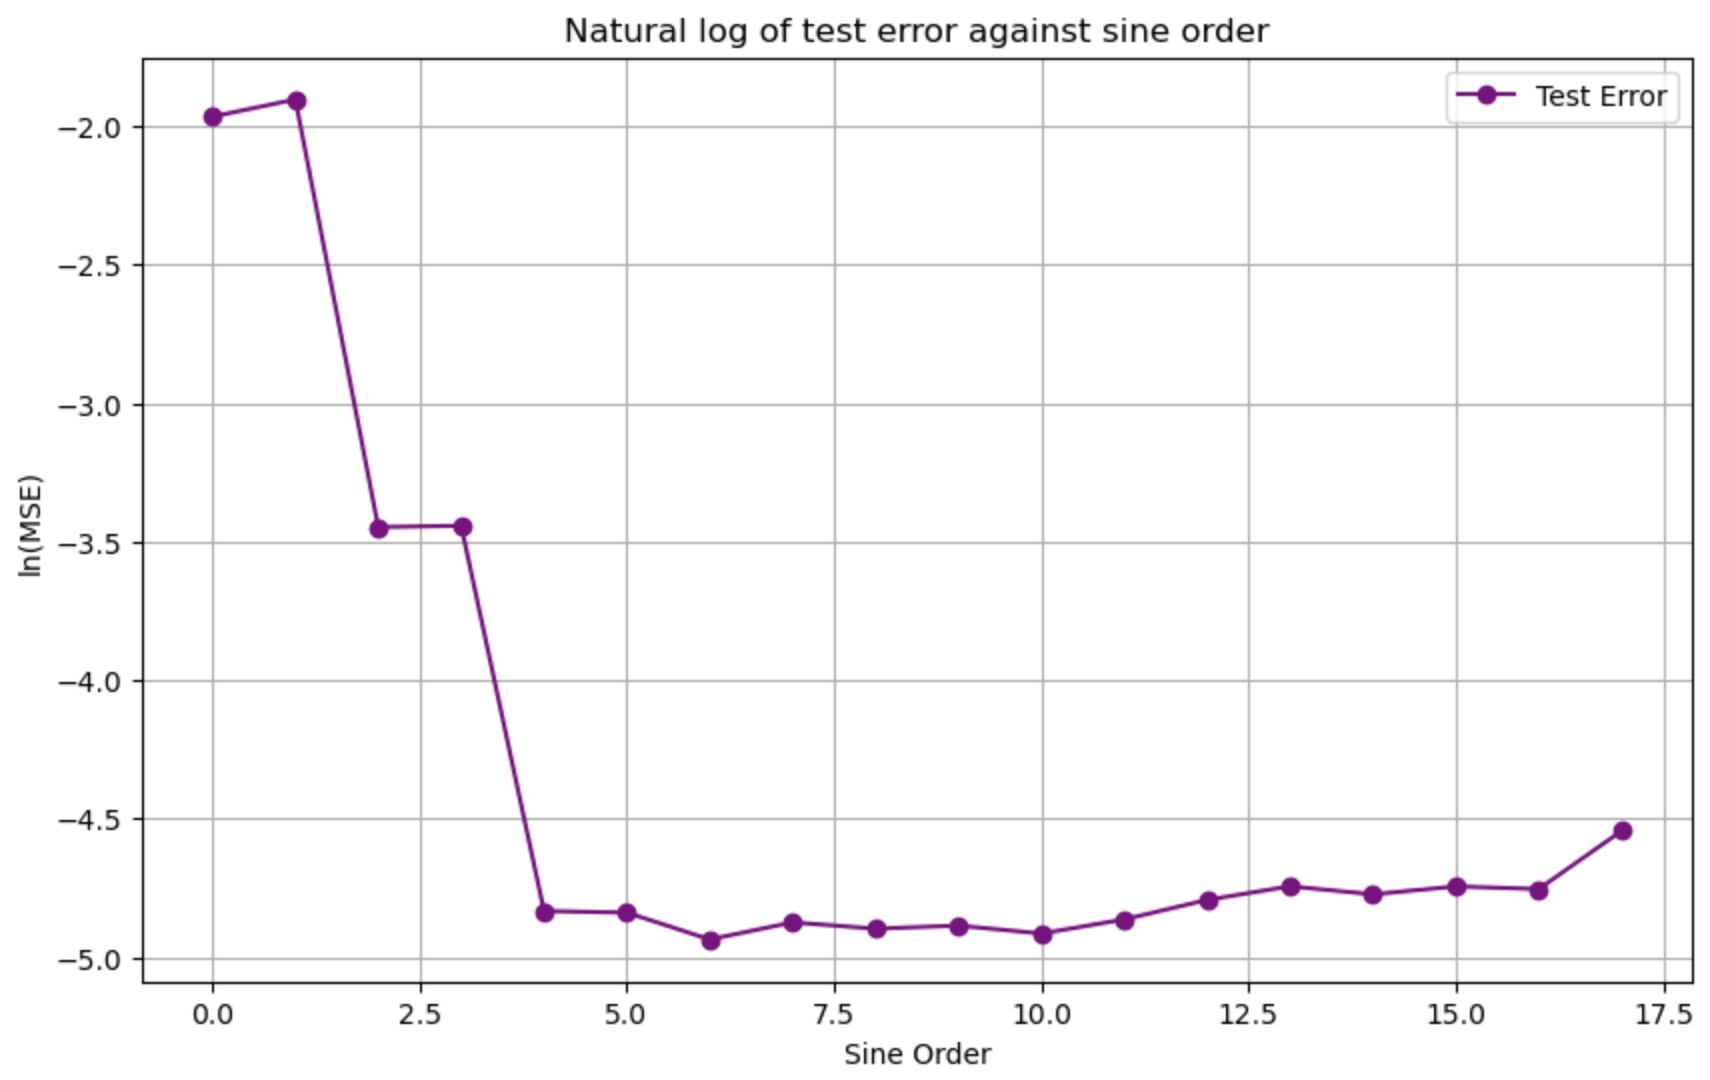
\includegraphics[width=0.7\textwidth]{images/question_3c.png}
        \caption{Figure showing the plot showing the test error against the order of the sine basis}
        \label{fig:question_3c}
    \end{figure}

    \begin{figure}[H]
        \centering
        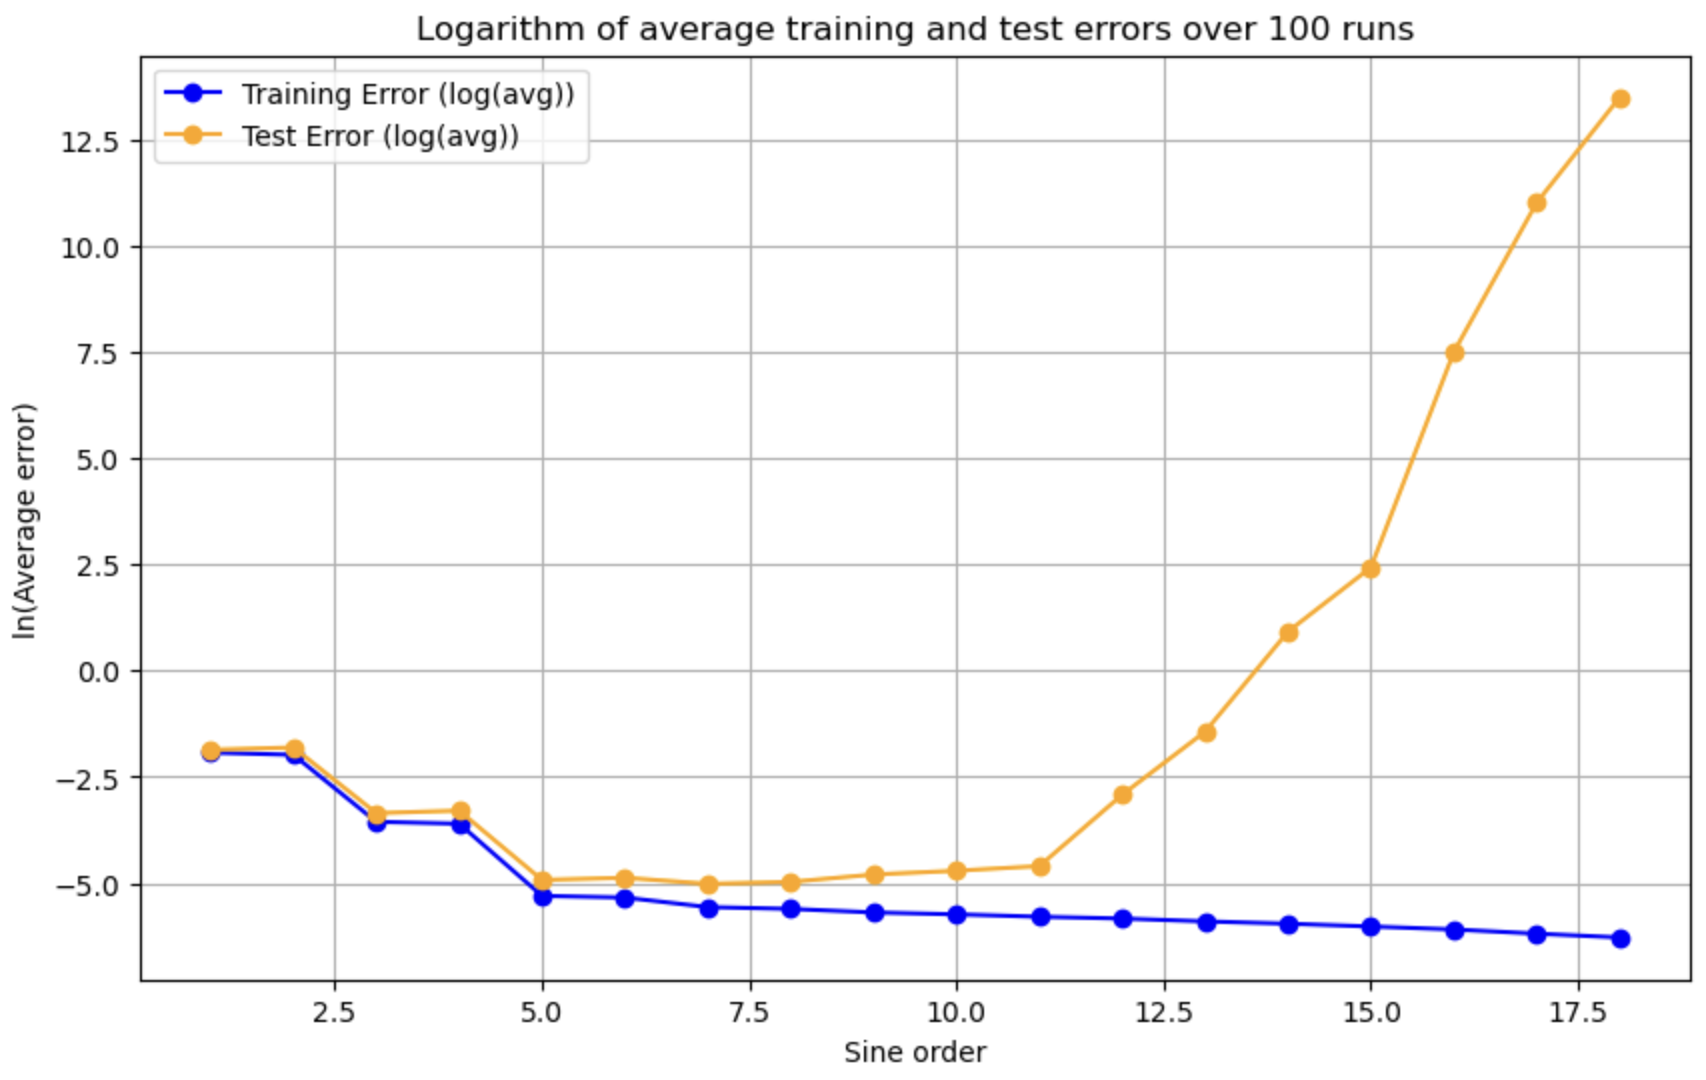
\includegraphics[width=0.7\textwidth]{images/question_3d.png}
        \caption{Figure showing the average result for the training and test errors using a sine basis over 100 runs}
        \label{fig:question_3d}
    \end{figure}
\end{enumerate}

\subsection{Filtered Boston housing and kernels}

\begin{enumerate}
    \item Predicting with the mean y-value on the training set. This is the naive regression of fitting the data with a constant function. The performance metrics of this method are shown in Table \ref{tab:question_4a}
    \begin{table}[H]
        \centering
        \begin{tabular}{ll}
            \hline
            \textbf{Metric} & \textbf{Value} \\
            \hline
            Average Training MSE & $83.4062 \pm 3.5878$ \\
            Average Test MSE & $86.7254 \pm 7.2282$ \\
           \hline
        \end{tabular}
        \caption{Naive Regression Performance Metrics}
        \label{tab:question_4a}
    \end{table}

    \item A simple interpretation of the constant function used in the previous question is that it is the mean of the median house price, the values we are trying to predict. 
    
    \item Predicting with a single attribute and a bias term. Increasing the complexity from the naive regression, we performed linear regression for each attribute. The resulting training and test Mean Squared Errors are shown in Table \ref{tab:question_4c}:

    \begin{table}[H]
        \centering
        \begin{tabular}{lll}
            \toprule
            \textbf{Feature} & \textbf{Training MSE} & \textbf{Test MSE} \\
            \midrule
            CRIM      & $70.8739 \pm 3.2060$ & $74.0706 \pm 6.5122$ \\
            ZN        & $72.4775 \pm 3.7925$ & $75.8473 \pm 7.6186$ \\
            INDUS     & $63.5788 \pm 3.6801$ & $67.3057 \pm 7.4810$ \\
            CHAS      & $81.3323 \pm 3.6556$ & $83.6017 \pm 7.5402$ \\
            NOX       & $67.7105 \pm 3.6276$ & $71.9494 \pm 7.3677$ \\
            RM        & $43.7150 \pm 3.4237$ & $43.6715 \pm 6.8463$ \\
            AGE       & $70.9769 \pm 3.8339$ & $75.8011 \pm 7.7557$ \\
            DIS       & $77.9363 \pm 3.9469$ & $82.0467 \pm 7.9962$ \\
            RAD       & $71.4678 \pm 3.7423$ & $73.8613 \pm 7.6423$ \\
            TAX       & $65.0696 \pm 3.6075$ & $67.9269 \pm 7.3778$ \\
            PTRATIO   & $62.9703 \pm 3.3148$ & $62.4538 \pm 6.6573$ \\
            LSTAT     & $37.7805 \pm 1.8333$ & $40.2146 \pm 3.8145$ \\
            \bottomrule
        \end{tabular}
        \caption{Single attribute regressions performance metrics}
        \label{tab:question_4c}
    \end{table}
    
    \item Predicting with all the attributes. The training and test MSE after using all the data at once are given in Table \ref{tab:question_4d}:

    \begin{table}[H]
        \centering
        \begin{tabular}{ll}
            \toprule
            \textbf{Metric} & \textbf{Value} \\
            \midrule
            Average Training MSE & $22.0224 \pm 1.7731$ \\
            Average Test MSE & $24.2901 \pm 3.7192$ \\
            \bottomrule
        \end{tabular}
        \caption{All attributes regression performance metrics}
        \label{tab:question_4d}
    \end{table}

    These results outperform the ones from the previous questions as required. 
\end{enumerate}

\subsection{Kernelised ridge regression}

\begin{enumerate}
    \item The BostonHousingAnalysis class in the jupyter notebook achieves the implementation of Kernel Ridge Regression using a Gaussian Kernel. As required it: initialises the hyperparameter vectors, performs kernel ridge regression with cross-validation, selects the optimal hyperparameters, retrains and evaluates the model with the MSE of the training and test sets. For the detail of the implementation, please refer to the comments in the code. 

    \item  The plot of the cross-validation error as a function of $\gamma$ and $\sigma$ is shown in Figure \ref{fig:question_5}:

    \begin{figure}[H]
        \centering
        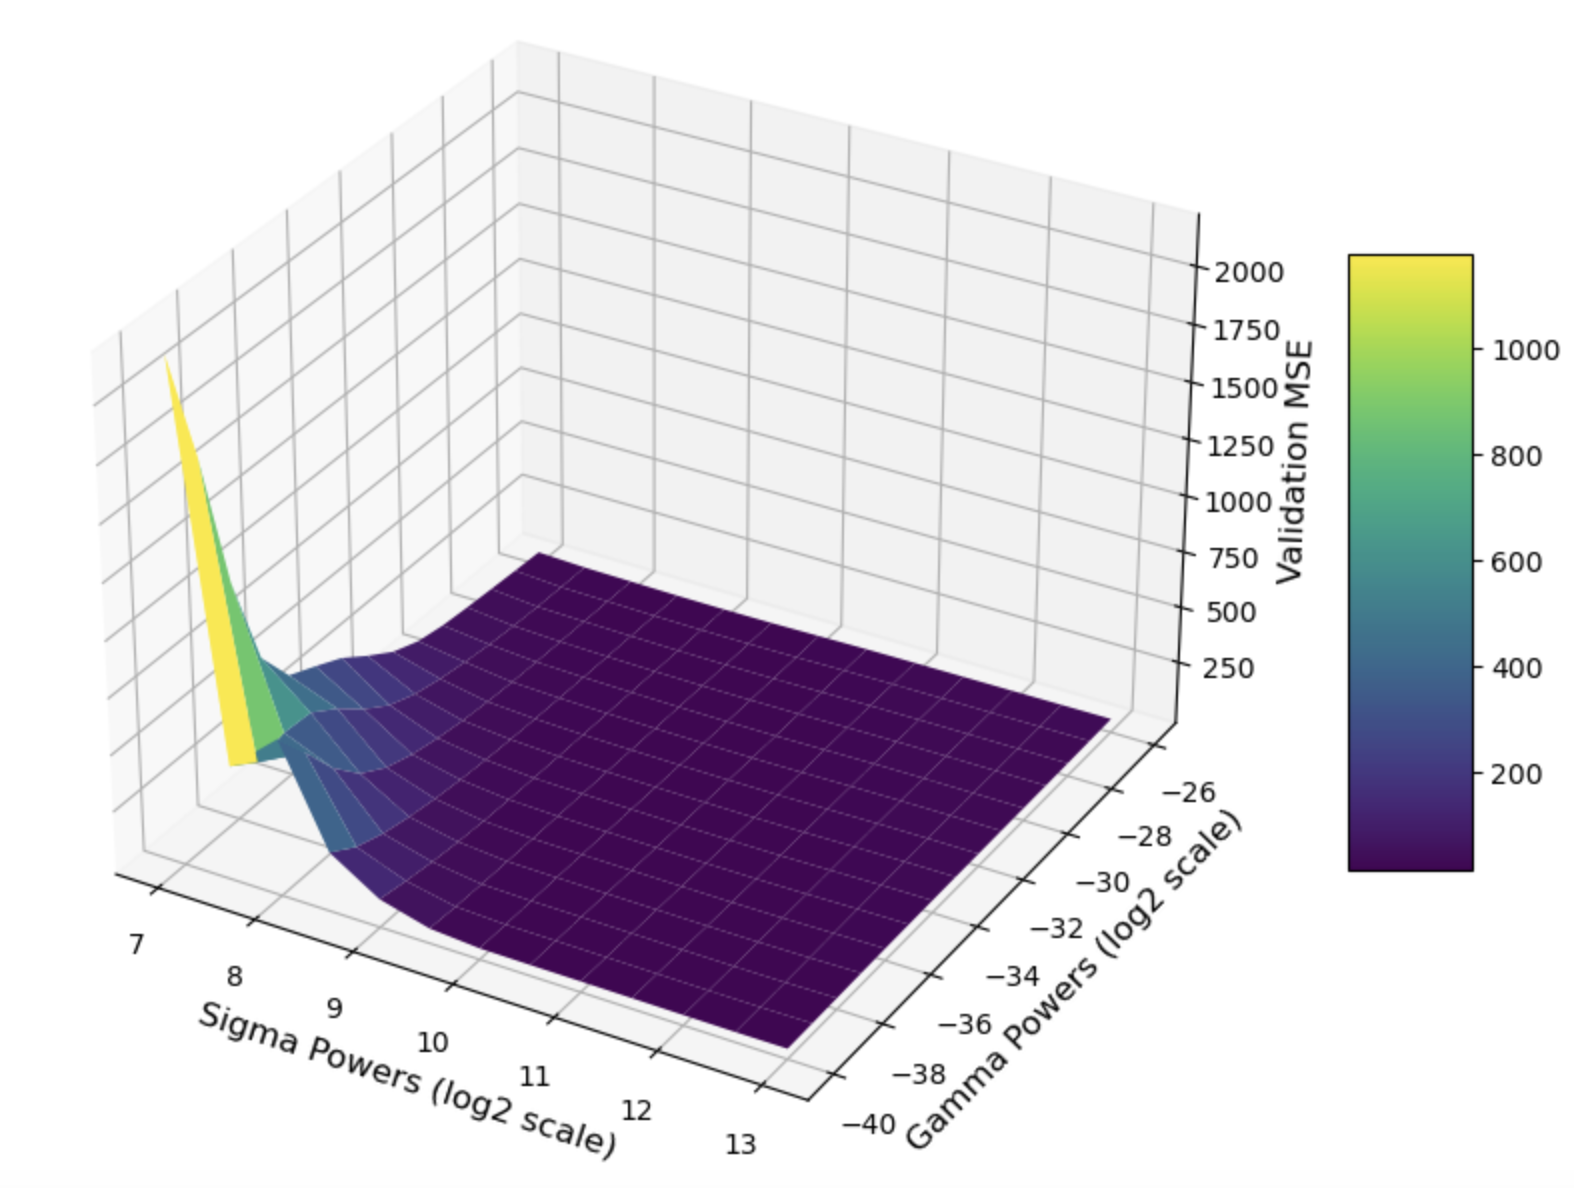
\includegraphics[width=0.7\textwidth]{images/question_5.png}
        \caption{Figure showing the cross-validation error as a function of $\gamma$ and $\sigma$}
        \label{fig:question_5}
    \end{figure}

    \item The Mean Squared Error on the training and test sets for the best $\gamma$ and $\sigma$ are: 
    \begin{enumerate}
        \item Training MSE: $8.137205$
        \item Test MSE: $14.22324$
    \end{enumerate}
    Note that the results saved in the jupyter notebook aren't the ones that were used in this question. The output of the BostonHousingAnalysis class used in section is given in the appendix. 

    \item The summary of the results obtained from repeating questions 4a, c and d as well as questions 5 a and c over 20 random (2/3, 1/3) splits of your data are recorded in Table \ref{tab:question_5d}:

    \begin{table}[H]
        \centering
        \begin{tabular}{|l|c|c|}
        \hline
        \textbf{Method} & \textbf{MSE train} & \textbf{MSE test} \\
        \hline
        Naive Regression & $86.1283 \pm 4.5339$ & $81.2697 \pm 8.9661$ \\
        \hline
        Linear Regression (CRIM) & $73.0630 \pm 4.8533$ & $70.2882 \pm 10.6816$ \\
        Linear Regression (ZN) & $75.0737 \pm 4.2831$ & $70.7135 \pm 8.6247$ \\
        Linear Regression (INDUS) & $66.5390 \pm 4.3773$ & $61.3513 \pm 8.8134$ \\
        Linear Regression (CHAS) & $83.1194 \pm 4.2663$ & $79.9543 \pm 8.6215$ \\
        Linear Regression (NOX) & $70.8872 \pm 4.6983$ & $65.6442 \pm 9.3682$ \\
        Linear Regression (RM) & $44.9055 \pm 1.9245$ & $41.3390 \pm    3.9541$ \\
        Linear Regression (AGE) & $74.3430 \pm 4.9046$ & $69.0054 \pm 9.8700$ \\
        Linear Regression (DIS) & $81.0787 \pm 4.7725$ & $75.7129 \pm 9.5114$ \\
        Linear Regression (RAD) & $73.8426 \pm 4.8299$ & $69.0242 \pm 9.5654$ \\
        Linear Regression (TAX) & $67.8265 \pm 4.3736$ & $62.3734 \pm   8.6025$ \\
        Linear Regression (PTRATIO) & $63.6893 \pm 3.5393$ & $60.9643 \pm 7.0877$ \\
        Linear Regression (LSTAT) & $39.0384 \pm 2.1745$ & $37.7584 \pm 4.2145$ \\
        \hline
        Linear Regression (all attributes) & $22.6646 \pm 1.1973$ & $23.3374 \pm 2.5949$ \\
        \hline
        Kernel Ridge Regression & $8.1372 \pm 1.5090$ & $14.2232 \pm    8.0884$ \\
        \hline
        \end{tabular}
    \caption{Table showing the mean squared error for various regression methods}
    \label{tab:question_5d}
    \end{table}

\end{enumerate}

\section{Part 2}

\begin{enumerate}
    \subsection{k-Nearest Neighbors}
        \subsubsection{Generating the data}

            Here is the obtained h function, and the associated decision regions (in blue and in red on the figure). You'll find in the attached code the used to obtain this result.

            \begin{figure}[H] % Position de l'image : 'h!' tente de placer l'image ici
                \centering % Centrage de l'image
                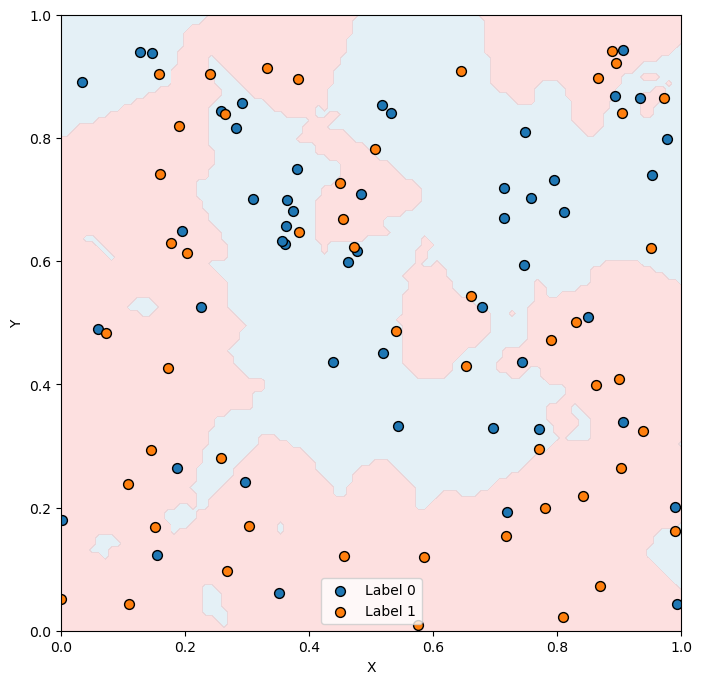
\includegraphics[width=0.7\textwidth]{images/image_part2.png}
                \caption{Visualization of a hypothesis $h_{100,3}$} % Légende sous l'image
                \label{fig:image1} % Étiquette pour faire référence à l'image dans le texte
            \end{figure}

        \subsubsection{Estimated generalization error of k-NN as a function of k}

        We used the attached code, and obtained the following plot. We updated the previous algorithms to work as much as possible with matrices to minimize the computation time.\\
        
        For k in {1,2,3,4, 5, 6}, the generalization error is very important, which is logical as we do not inspect a sufficient amount of data to estimate correctly the label of our new data point : we are here subject to overfitting and are capturing the noise in our training dataset (we notice that for k={1,2}, our generalization error is close to 0.2, which is the proportion of the noise in our data). Then, for k between 7 and 15, our average generalization error is minimal : we inspect enough training points to avoid overfitting, and sufficiently few training points to stay close to the point we want to evaluate and capture the local pattern. For k>15, the generalization error increases : we are looking at data points situated too far away from the one we are trying to evaluate, and end up misclassifying it.\\

        \begin{figure}[H] % Position de l'image : 'h!' tente de placer l'image ici
            \centering % Centrage de l'image
            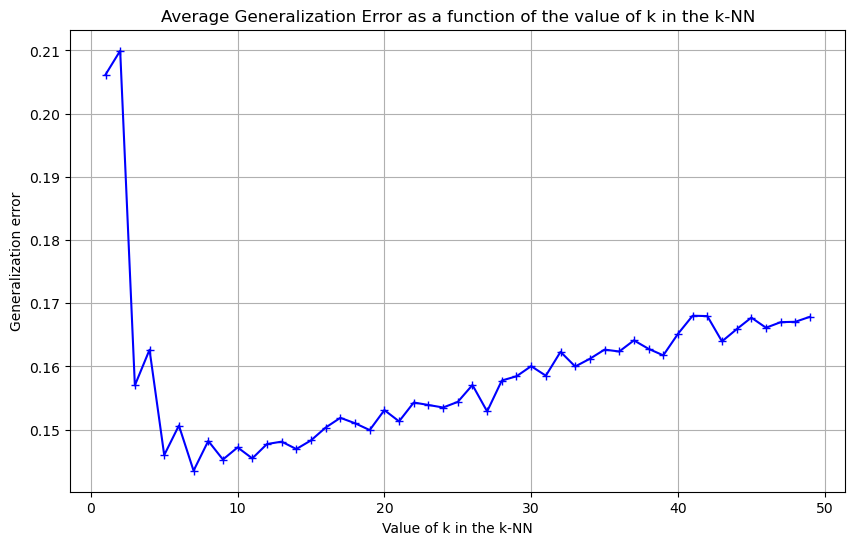
\includegraphics[width=0.9\textwidth]{images/image_part2_2.png}
            \caption{Average Generalization Error as a function of the value of k in the k-NN} % Légende sous l'image
            \label{fig:image1} % Étiquette pour faire référence à l'image dans le texte
        \end{figure}\\

    \subsubsection{Determine the optimal k as a function of the number of training points (m)}
    
        We used the attached code, and obtained the following plot. We changed the previous algorithms to work as much as possible with matrices to minimize the computation time.\\

        We notice that the more samples we have, the bigger our optimal k is. This result seems logical : the more training samples we have, the more noisy data (in absolute number) we have. We therefore need to look at more neighbours to estimate our label correctly. In other words, the more training samples we have, the more complex/dense our decision space is and the more difficult our decision is to make : the consequence is that we need to look at more neighbours to make an accurate decision. We can also notice that this curve tends to flatten for $k\geq1500$, which is explained by the fact that when we already inspect a large number of neighbours, the additional value of having more is relatively low : we already manage to capture the local pattern with the neighbours that we are inspecting. \\


        \begin{figure}[H] % Position de l'image : 'h!' tente de placer l'image ici
            \centering % Centrage de l'image
            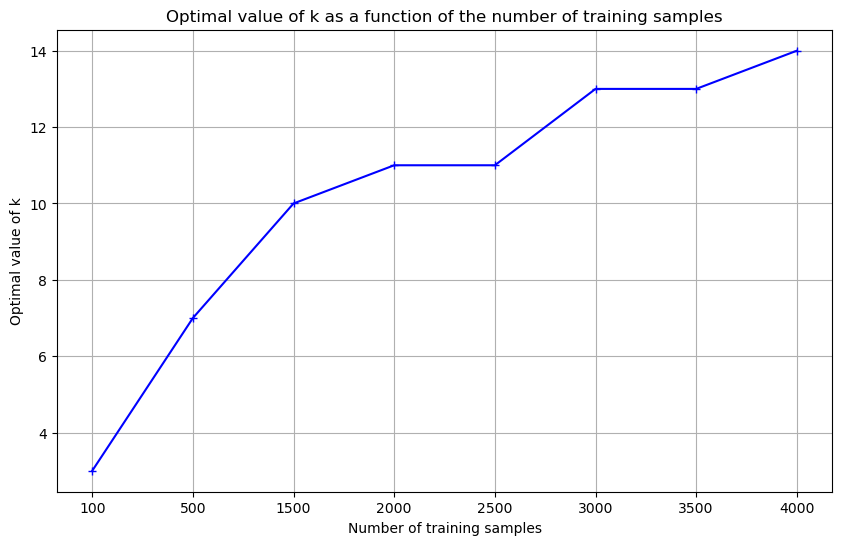
\includegraphics[width=0.9\textwidth]{images/image_part2_3.png}
            \caption{Optimal value of k as a function of the number of training samples} % Légende sous l'image
            \label{fig:image1} % Étiquette pour faire référence à l'image dans le texte
        \end{figure}
\end{enumerate}

\section{Part 3}
\begin{enumerate}
    \item Question 9
        \begin{enumerate}
        \item Let's fix $\{x_1, ..., x_n\}$ a family of vectors of $R^n$. $\forall i \in \llbracket 1,n \rrbracket$ we have $x_i = [x_{i1}, x_{i2},..., x_{in}]^T $ Let's write K, the Kernel matrix associated with this family. We have : 
\\
\[
K = \begin{bmatrix}
  c + \sum_{i=1}^n x_{1i}^T x_{1i} & \cdots & c + \sum_{i=1}^n x_{ni}^T x_{1i} \\
  \vdots & \ddots & \vdots \\
  c + \sum_{i=1}^n x_{1i}^T x_{ni} & \cdots & c + \sum_{i=1}^n x_{ni}^T x_{ni}
\end{bmatrix}
\]
\\
\[
\implies K = c \begin{bmatrix}
  1 & \cdots & 1 \\
  \vdots & \ddots & \vdots \\
  1 & \cdots & 1
\end{bmatrix} + \begin{bmatrix}
  \sum_{i=1}^n x_{1i}^T x_{1i} & \cdots & \sum_{i=1}^n x_{ni}^T x_{1i} \\
  \vdots & \ddots & \vdots \\
  \sum_{i=1}^n x_{1i}^T x_{ni} & \cdots & \sum_{i=1}^n x_{ni}^T x_{ni}
\end{bmatrix}
\]\\

$\forall (x,z) \in (R^n)^2 , K_c(x, z)$ is a kernel if and only if K is Positive Semi Definite : $K_c(x, z)$ is a  kernel if and only if $\forall z \in R^n, z^TKz \geq 0$. Let's fix $ z \in R^n$. \\

\[
 z^TKz = c z^T\begin{bmatrix}
  1 & \cdots & 1 \\
  \vdots & \ddots & \vdots \\
  1 & \cdots & 1
\end{bmatrix}z + z^T\begin{bmatrix}
  \sum_{i=1}^n x_{1i}^T x_{1i} & \cdots & \sum_{i=1}^n x_{ni}^T x_{1i} \\
  \vdots & \ddots & \vdots \\
  \sum_{i=1}^n x_{1i}^T x_{ni} & \cdots & \sum_{i=1}^n x_{ni}^T x_{ni}
\end{bmatrix}z
\]\\

\[ \implies
 z^TKz = c [\sum_{i=1}^nz_i,\cdots, \sum_{i=1}^nz_i]z + [\sum_{l=1}^n z_l \sum_{i=1}^n x_{1i}^T x_{li}, \cdots, \sum_{l=1}^n z_l \sum_{i=1}^n x_{ni}^T x_{li}]z
\]\\

\[ \implies
 z^TKz = c \sum_{i=1}^n z_i \sum_{l=1}^n z_l + \sum_{j=1}^n z_j \sum_{l=1}^n z_l \sum_{i=1}^n x_{ji}^T x_{li}
\]\\

\[ \implies
 z^TKz = c \big(\sum_{i=1}^n z_i\big)^2 + \sum_{j=1}^n  \sum_{l=1}^n  \sum_{i=1}^n z_jx_{ji}^T z_lx_{li}
\]\\

We have finally : \\

\[  z^TKz \geq 0 \implies c \big(\sum_{i=1}^n z_i\big)^2 + \sum_{j=1}^n  \sum_{l=1}^n  \sum_{i=1}^n z_jx_{ji}^T z_lx_{li} \geq 0 \]\\

\[
\implies c \geq \frac{-\sum_{j=1}^n  \sum_{l=1}^n  \sum_{i=1}^n z_jx_{ji}^T z_lx_{li}}{\big(\sum_{i=1}^n z_i\big)^2}
\]\\

    \item c is a regularizer, it allow to take into consideration rather equally all the training datapoints when making a new prediction, instead of only using training datapoints that are similar to the points we want to classify.

    The kernel can be rewritten : $ K_c (x,z) = c + \langle \mathbf{x}, \mathbf{z} \rangle$. Therefore, if x and z point in the same direction, the value of $ K_c (x,z)$ is greater, and x have a more important weight in the value predicted for z. We remark that if x and z are orthogonal, x will have a null weight and will therefore have no impact in the value predicted for z. Those phenomenons result in the fact that we only use a subset of our training points (the ones that are similar to the data we want to classify) to classify our new data, which could lead to misclassifications.\\

    If c is very big, the impact of this phenomenon is reduced : an important value of c allows to reduce the contribution of the scalar product in the weight given to a training datapoint. Hence, all datapoints participate rather uniformly in the classification of the new points.
        \end{enumerate}

    \item Question 10 : \\
    
    We can write our prediction function as follows :

\[
f(t) = \sum_{i=1}^m \alpha_iK_{\beta}(x_i,t)
\]\\

We know that $\alpha = K^{-1}y$ with y the labels of our target, and K the following matrix : \[
K = \begin{bmatrix}
  e^{-\beta \lVert x_1 - x_1 \rVert} & ... & e^{-\beta \lVert x_1 - x_m \rVert} \\
  ... & ... & ... \\
  e^{-\beta \lVert x_1 - x_m \rVert} & ... & e^{-\beta \lVert x_m - x_m \rVert} \\
\end{bmatrix} = \begin{bmatrix}
  1 & ... & e^{-\beta \lVert x_1 - x_m \rVert} \\
  ... & 1 & ... \\
  e^{-\beta \lVert x_1 - x_m \rVert} & ... & 1 \\
\end{bmatrix}
\]\\

We notice that if $\beta >> 0$, $K = I = K^{-1}$. We have therefore the following prediction function : \\

\[
f(t) = \sum_{i=1}^m \alpha_iK_{\beta}(x_i,t) = \sum_{i=1}^m sign(y_i)K_{\beta}(x_i,t)
\]\\

If we assume, for simplicity, that our nearest neighbor is the first one (i=1), we can rewrite our prediction function : \\

\[
f(t) = sign(y_1)K_{\beta}(x_1,t) + \sum_{i=2}^m sign(y_i)K_{\beta}(x_i,t)
\]\\

If $sign(y_1)>0$, we need to have sign(f(t))>0, which implies : 

\[
sign(y_1)K_{\beta}(x_1,t) + \sum_{i=2}^m sign(y_i)K_{\beta}(x_i,t) > 0 \implies e^{-\beta\lVert x_1-t \rVert^{2}} > -\sum_{i=2}^m sign(y_i)e^{-\beta \lVert x_i-t \rVert^{2}}
\]\\

Similarly, if $sign(y_1)<0$, we need to have sign(f(t))<0, which implies : 

\[
sign(y_1)K_{\beta}(x_1,t) + \sum_{i=2}^m sign(y_i)K_{\beta}(x_i,t) < 0 \implies -e^{-\beta\lVert x_1-t \rVert^{2}} < -\sum_{i=2}^m sign(y_i)e^{-\beta \lVert x_i-t \rVert^{2}}
\]
\[ \implies e^{-\beta\lVert x_1-t \rVert^{2}} > \sum_{i=2}^m sign(y_i)e^{-\beta \lVert x_i-t \rVert^{2}}
\]\\

Then, we have this inequality : 

\[ e^{-\beta\lVert x_1-t \rVert^{2}} > | \sum_{i=2}^m sign(y_i)e^{-\beta \lVert x_i-t \rVert^{2}}|
\]\\

Finally, if we write $\epsilon_i = e^{-\beta \lVert x_i-t \rVert^2}$, we obtain this equation on beta : 

\[ e^{-\beta\lVert x_1-t \rVert^{2}} > | \sum_{i=2}^m sign(y_i)\epsilon_i|
\]\\

To conclude, if $\beta$ satisfies the previous inequality, our classifier can be assimilated to a 1-Nearest Neighbor.\\

    \item Question 11
    \begin{enumerate}
        \item 
 \[\mathcal{E}_{\rho_i}(f_i) = \int_{\mathcal{X, Y}} \mathbb{1}_{ \{f_i(x) \neq y\} } d\rho_i(x, y)\]

\[ \implies
\mathcal{E}_{\rho_i}(f_i) = \int_{\mathcal{X, Y}} \mathbb{1}_{ \{f_i(x) \neq y\} } \rho_i(x, y) dxdy = \int_{\mathcal{X, Y}} \mathbb{1}_{\{f_i(x) \neq y\} } \mathbb{1}_{\{f_i(x) = y\}} \frac{1}{2n} dxdy
\]\\

We remark that $\mathbb{1}_{ \{f_i(x) \neq y\} } \mathbb{1}_{\{f_i(x) = y\}}$ = 0, and deduce that $\mathcal{E}_{\rho_i}(f_i)$ = 0 \\

Since the misclassification excess risk is always positive, we have : 

\[ 0= \mathcal{E}_{\rho_i}(f_i) \geq \inf_{f : \mathcal{X} \rightarrow \mathcal{Y}} \mathcal{E}_{\rho_i}(f) \geq 0 \implies \mathcal{E}_{\rho_i}(f_i) = \inf_{f : \mathcal{X} \rightarrow \mathcal{Y}} \mathcal{E}_{\rho_i}(f) = 0
\]\\

\item

Let's first show that $ E_{S \sim \rho_i^n}(\mathcal{E}_{\rho}(A(S))) = \frac{1}{k}\sum_{i=1}^{T} \mathcal{E}_{\rho_i}(A(S_j^i))$, for any $i \in \{1, ..., T\}$\\

For any $i \in \{1, ..., T\}$, we can write :

\[
\mathcal{E}_{\rho_i}(A(S)) = \int_{\mathcal{X}, \mathcal{Y}} \mathbb{1}_{\{A(S)(x)\neq y\}} d\rho_i(x,y) = \int_{\mathcal{X}, \mathcal{Y}} \mathbb{1}_{\{A(S)(x)\neq y\}} \mathbb{1}_{\{f_i(x) = y\}} \frac{1}{2n}dxdy
\]\\

We notice that $\mathbb{1}_{ \{ A(S)(x)\neq y \} } \mathbb{1}_{\{f_i(x) = y\}} = 0$ for (x,y) $\notin (S_j^i)_{j\in \{1, k\}}$, which means that we are constrained in the values that S can take as inputs.\\

Our previous equation can be rewritten :

\[
\mathcal{E}_{\rho_i}(A(S)) = \int_{(x,y)\in (S_j^i)_{j\in \{1, k\}} } \mathbb{1}_{\{A(S_j^i)(x)\neq y\}} \mathbb{1}_{\{f_i(x) = y\}} dxdy
\]\\
\[ \implies
\mathcal{E}_{\rho_i}(A(S)) = \mathcal{E}_{\rho_i}(A(S)_{| (x,y)\in (S_j^i)_{j\in \{1, k\}}}) = \mathcal{E}_{\rho_i}((S_j^i)_{j\in \{1, k\}})
\]\\

We have an equal probability of sampling each one of the k sets, which gives: 

\[
E_{S \sim \rho_i^n} \mathcal{E}_{\rho_i}(A(S)) = \mathcal{E}_{\rho_i}((S_j^i)_{j\in \{1, k\}}) = \frac{1}{k} \sum_{j=1}^k \mathcal{E}_{\rho_i}(A(S_j^i))
\]\\

We use the fact that $\max_m \alpha_m \geq \frac{1}{m} \sum_{\ell=1}^{m} \alpha_m$ to deduce that, one one hand we have :

\[
\max_{\{i=1, ..., T\}}E_{S \sim \rho_i^n} \mathcal{E}_{\rho_i}(A(S))\geq \frac{1}{T} \sum_{i=1}^T E_{S \sim \rho_i^n} \mathcal{E}_{\rho_i}(A(S)) = \frac{1}{T} \sum_{i=1}^T\frac{1}{k} \sum_{j=1}^k \mathcal{E}_{\rho_i}(A(S_j^i))
\]\\

We then use the fact that $\frac{1}{m} \sum_{\ell=1}^{m} \alpha_m \geq \min_m \alpha_m$ to deduce that on the other hand we have :

\[
\frac{1}{T} \sum_{i=1}^T\frac{1}{k} \sum_{j=1}^k \mathcal{E}_{\rho_i}(A(S_j^i)) = \frac{1}{k} \sum_{j=1}^k\frac{1}{T} \sum_{i=1}^T \mathcal{E}_{\rho_i}(A(S_j^i)) \geq \min_{\{j=1, ..., k\}} \frac{1}{T} \sum_{i=1}^T \mathcal{E}_{\rho_i}(A(S_j^i)) 
\]\\

If we unite our inequalities together, we obtain the demanded result : \\

\[
\max_{\{i=1, ..., T\}}E_{S \sim \rho_i^n} \mathcal{E}_{\rho_i}(A(S))\geq\frac{1}{T} \sum_{i=1}^T\frac{1}{k} \sum_{j=1}^k \mathcal{E}_{\rho_i}(A(S_j^i)) \geq \min_{\{j=1, ..., k\}} \frac{1}{T} \sum_{i=1}^T \mathcal{E}_{\rho_i}(A(S_j^i)) 
\]\\

\[ \implies
\max_{\{i=1, ..., T\}}E_{S \sim \rho_i^n} \mathcal{E}_{\rho_i}(A(S)) \geq \min_{\{j=1, ..., k\}} \frac{1}{T} \sum_{i=1}^T \mathcal{E}_{\rho_i}(A(S_j^i)) 
\]\\

\item We have : 

\[
\frac{1}{T} \sum_{i=1}^{T} \mathcal{E}_{\rho_i}(A(S_j^i)) =  \frac{1}{T} \sum_{i=1}^{T} \int_{\mathcal{X}, \mathcal{Y}} \mathbb{1}_{\{A(S_i^j)(x) \neq y\}} d\rho_i(x,y) = \frac{1}{T} \sum_{i=1}^{T} \int_{\mathcal{X}, \mathcal{Y}} \mathbb{1}_{\{A(S_i^j)(x) \neq y\}} \mathbb{1}_{\{f_i(x) = y\}} \frac{1}{2p} dxdy
\]
\[ \implies
\frac{1}{T} \sum_{i=1}^{T} \mathcal{E}_{\rho_i}(A(S_j^i)) = \frac{1}{T} \sum_{i=1}^{T} \int_{\mathcal{X}, \mathcal{Y}} \mathbb{1}_{\{A(S_i^j)(x) \neq y\}} \mathbb{1}_{\{f_i(x) = y\}} \frac{1}{2p} dxdy
\]\\

We notice that $\mathbb{1}_{\{A(S_i^j)(x) \neq y\}} \mathbb{1}_{\{f_i(x) = y\}} = \mathbb{1}_{\{A(S_i^j)(x) \neq f_i(x)\}}$\\

We can rewrite our previous expression : 

\[
\frac{1}{T} \sum_{i=1}^{T} \mathcal{E}_{\rho_i}(A(S_j^i)) = \frac{1}{T} \sum_{i=1}^{T} \int_{\mathcal{X}, \mathcal{Y}} \frac{1}{2p} \mathbb{1}_{\{A(S_i^j)(x) \neq f_i(x)\}} dxdy
\]

We then notice that for $x \in S_j^i$, $\mathbb{1}_{\{A(S_i^j)(x) \neq f_i(x)\}} = 0$. Our integral can therefore be rewritten : 

\[
\frac{1}{T} \sum_{i=1}^{T} \mathcal{E}_{\rho_i}(A(S_j^i)) = \frac{1}{T} \sum_{i=1}^{T} \int_{R_j} \frac{1}{2p} \mathbb{1}_{\{A(S_i^j)(x) \neq f_i(x)\}} dx = \frac{1}{T} \sum_{i=1}^{T}\sum_{v\in R_j} \frac{1}{2p} \mathbb{1}_{\{A(S_i^j)(v) \neq f_i(v)\}}
\]

We then use the fact that $\frac{1}{m}\sum_{l=1}^m\alpha_m \geq \min_{l=1,\dots,m} \alpha_m$ to obtain : 

\[
\frac{1}{T} \sum_{i=1}^{T} \mathcal{E}_{\rho_i}(A(S_j^i)) = \frac{1}{2}\frac{1}{p}\sum_{v\in R_j}  \frac{1}{T} \sum_{i=1}^{T} \mathbb{1}_{\{A(S_i^j)(v) \neq f_i(v)\}} \geq \frac{1}{2} \min_{v\in\mathcal{R_j}}\sum_{i=1}^{T} \mathbb{1}_{\{A(S_i^j)(v) \neq f_i(v)\}}
\]\\

The previous inequality gives the final result :

\[
\frac{1}{T} \sum_{i=1}^{T} \mathcal{E}_{\rho_i}(A(S_j^i)) \geq \frac{1}{2} \min_{v\in\mathcal{R_j}}\sum_{i=1}^{T} \mathbb{1}_{\{A(S_i^j)(v) \neq f_i(v)\}}
\]\\

\item 
First, we will prove that for any v $\in R_j$ we can partition $\mathcal{Y}^{\mathcal{C}}$ into $\frac{T}{2}$ pairs $(f_i, f_{i'})$ such that $f_i(x) \neq f_{i'}(x)$ if and only if x = v.  To prove this, we will prove that : for any v $\in R_j$ we can partition $\mathcal{Y}^{\mathcal{C}}$ into $\frac{T}{2}$ pairs $(f_i, f_{i'})$ such that $f_i(x) = f_{i'}(x)$ if and only if x $\neq$ v.\\

First, for a fixed $x \in \mathcal{C}$, we assume that there exist $(fi', fi'') \in (\mathcal{Y}^C)^2 $ so that x=v if and only if $f_i(x) = f_{i'}(x)=f_{i''}(x)$, Therefore, if x $\neq$ v, we have $f_i(x) \neq f_{i'}(x)$ and $f_i(x) \neq f_{i''}(x)$. Those three functions take their values in $\{-1,1\}$, which implies that if we have $f_i(x) \neq f_{i'}(x)$ and $f_i(x) \neq f_{i''}(x)$ at the same time, we automatically have $\forall i \in C, f_{i''}(x) = f_{i'}(x) \Leftrightarrow f_{i''} = f_{i'}$.\\

Hence, there is one only one $i' \in \llbracket 1,T \rrbracket $ so that x $\neq$ v if and only if $f_i(x) = f_{i'}(x)$. \\

We proved that for any v $\in R_j$ we can partition $\mathcal{Y}^{\mathcal{C}}$ into $\frac{T}{2}$ pairs $(f_i, f_{i'})$ such that $f_i(x) \neq f_{i'}(x)$ if and only if x = v.\\

Now, let's consider one par $(f_i, f_{i'})$, and v $\in R_j$. Let's also consider $\mathbb{1}_{\{A(S_j^i)(v) \neq f_i(v)\}} + \mathbb{1}_{\{A(S_j^{i'})(v) \neq f_{i'}(v)\}}$. Since $A(S_j^i)(v) = A(S_j^{i'})(v)$ and $f_i(v) \neq f_{i'}(v)$ one of the the terms will be 0, and the other will be 1. We have in any cases : $\mathbb{1}_{\{A(S_j^i)(v) \neq f_i(v)\}} + \mathbb{1}_{\{A(S_j^{i'})(v) \neq f_{i'}(v)\}} = 1$

Finally, we obtain the formula : 

\[
2 \sum_{i=1}^{T} \mathbb{1}_{\{A(S_j^i)(v) \neq f_i(v)\}} = \sum_{i=1}^{T} \mathbb{1}_{\{A(S_j^i)(v) \neq f_i(v)\}} + \sum_{i'=1}^{T}\mathbb{1}_{\{A(S_j^{i'})(v) \neq f_{i'}(v)\}} = T
\]\\

\[ \implies 
\frac{2}{T} \sum_{i=1}^{T} \mathbb{1}_{\{A(S_j^i)(v) \neq f_i(v)\}} = \frac{1}{T} \big( \sum_{i=1}^{T} \mathbb{1}_{\{A(S_j^i)(v) \neq f_i(v)\}} + \sum_{i'=1}^{T}\mathbb{1}_{\{A(S_j^{i'})(v) \neq f_{i'}(v)\}}\big) = 1
\]\\

\[ \implies 
\frac{1}{T} \sum_{i=1}^{T} \mathbb{1}_{\{A(S_j^i)(v) \neq f_i(v)\}} = \frac{1}{2}
\]\\
 \item 
For any random variable Z and a $\in \mathcal{R}_+^*$, Markov's inequality is the following : $P(Z \geq a) \leq \frac{E(A)}{a}$. \\

Let's apply this inequality to the positive random variable defined by A = $-\frac{Z-1}{b}$, with Z being random variable with values in [0, 1], b $\in ]0,1]$ and a = 1. We have : \\

\[ P( A\geq 1) \leq \frac{E(A)}{1} \implies P( -\frac{Z-1}{b}\geq 1) \leq -E\big(\frac{Z-1}{b}\big)
\]

\[ \implies P( Z-1 \leq -b) \leq -E\big(\frac{Z-1}{b}\big) \implies 1-P( Z-1 > -b) \leq -E\big(\frac{Z-1}{b}\big)
\]

\[ \implies 1-P( Z > 1-b) \leq -\frac{\mu-1}{b} \implies P( Z > 1-b) \geq \frac{\mu-1}{b} + 1 
\]
\[
\implies P( Z > 1-b) \geq \frac{\mu-(1-b)}{b}
\]
\\

\item 
We know that $\mathcal{E}_{\rho}(A(S))$ is a random variable taking values in [0,1]. For $i\in \llbracket 1,T\rrbracket,$ let's apply the inequality found in 11.e) to  Z=$\mathcal{E}_{\rho_i}(A(S))$ and a=$\frac{7}{8}$ : 

\[
 P_{S \sim \rho_i^n}( \mathcal{E}_{\rho_i}(A(S)) > 1-\frac{7}{8}) \geq \frac{E_{S \sim \rho_i^n}(\mathcal{E}_{\rho_i}(A(S)))-(1-\frac{7}{8})}{\frac{7}{8}}
\]
\[
 \Leftrightarrow P_{S \sim \rho_i^n}( \mathcal{E}_{\rho_i}(A(S)) > \frac{1}{8}) \geq \frac{8E_{S \sim \rho_i^n}(\mathcal{E}_{\rho_i}(A(S)))-1}{7}
\]\\

This inequality is true for all values of i, and in particular for $ i' = arg \max_{\{i=1, ..., T\}}E_{S \sim \rho_i^n} \mathcal{E}_{\rho_i}(A(S))$. We obtain for this case : \\ 

\[
 P_{S \sim \rho_i^n}( \mathcal{E}_{\rho_i}(A(S)) > \frac{1}{8}) \geq \frac{8E_{S \sim \rho_{i'}^n}(\mathcal{E}_{\rho_{i'}}(A(S)))-1}{7} = \frac{8\max_{\{i=1, ..., T\}}E_{S \sim \rho_{i}^n}(\mathcal{E}_{\rho_i}(A(S)))-1}{7}
\]\\

Next, we know from question 11.b that :

\[
\max_{\{i=1, ..., T\}}E_{S \sim \rho_i^n} \mathcal{E}_{\rho_i}(A(S)) \geq \min_{\{j=1, ..., k\}} \frac{1}{T} \sum_{i=1}^T \mathcal{E}_{\rho_i}(A(S_j^i)) 
\]\\

And from question 11.c that : \\
\[
\frac{1}{T} \sum_{i=1}^T \mathcal{E}_{\rho_i} \left( A(S_j^i) \right) \geq \frac{1}{2} \min_{v \in R_j} \frac{1}{T} \sum_{i=1}^T \mathbb{1}_{\{ A(S_j^i)(v) \neq f_i(v) \}}
\]\\

Hence, we have : \\
\[
\max_{\{i=1, ..., T\}}E_{S \sim \rho_i^n} \mathcal{E}_{\rho_i}(A(S)) \geq \min_{\{j=1, ..., k\}} \frac{1}{T} \sum_{i=1}^T \mathcal{E}_{\rho_i}(A(S_j^i)) \geq \min_{\{j=1, ..., k\}} \frac{1}{2} \min_{v \in R_j} \frac{1}{T} \sum_{i=1}^T \mathbb{1}_{\{ A(S_j^i)(v) \neq f_i(v) \}}
\]\\

Finally, we learned in question 11.d that : \\

\[
\frac{1}{T} \sum_{i=1}^T \mathbb{1}_{\{ A(S_j^i)(v) \neq f_i(v) \}} = \frac{1}{2}
\]\\

The previous equality gives us that : 

\[
\max_{\{i=1, ..., T\}}E_{S \sim \rho_i^n} \mathcal{E}_{\rho_i}(A(S))
\geq \min_{\{j=1, ..., k\}}\frac{1}{2} \min_{v \in R_j} \frac{1}{T} \sum_{i=1}^T \mathbb{1}_{\{ A(S_j^i)(v) \neq f_i(v) \}} = \frac{1}{2} \frac{1}{2} = \frac{1}{4}
\]

Finally, we obtain the inequality :

\[ P_{S \sim \rho_i^n}( \mathcal{E}_{\rho_i}(A(S)) > \frac{1}{8}) \geq \frac{8\max_{\{i=1, ..., T\}}E_{S \sim \rho_i^n}(\mathcal{E}_{\rho_i}(A(S)))-1}{7} \geq \frac{8\frac{1}{4}-1}{7} = \frac{1}{7}
\]\\

The previous inequality being true for all values of i, we obtain the demanded relation : 

\[ P_{S \sim \rho^n}( \mathcal{E}_{\rho}(A(S)>\frac{1}{8}) > \frac{1}{7}
\]\\


\item \begin{enumerate}
    \item We first demonstrated that : $\inf_{f : \mathcal{X} \rightarrow \mathcal{Y}} \mathcal{E}_{\rho}(f) = 0$. This result shows that, for each distribution $\rho$, there exists at least one function that minimizes the misclassification excess risk relative to that distribution. In other words, for any given machine learning problem defined by a distribution $\rho$, there is an ideal function or solution that can achieve minimal error.\\
    
    We then demonstrated that $P_{S \sim \rho^n}( \mathcal{E}_{\rho}(A(S)) > \frac{1}{8}) \geq \frac{1}{7}$. This means that, given a dataset sampled from the distribution $\rho$, the probability that the misclassification excess risk of any algorithm A will exceed $\frac{1}{8}$ is at least $\frac{1}{7}$. In other words, there is no universal algorithm that can guarantee low error across all possible datasets. Each algorithm’s performance depends on the specific distribution of the data, showing that no single algorithm can fit perfectly across all problems.\\
    
    The No Free Lunch theorem can therefore be expressed as follows: There exists an optimal solution function for each machine learning problem, but the solutions for two distinct problems are generally distinct. Consequently, there is no single algorithm that performs best on all possible problems; rather, different problems require different solutions. \\

    \item This theorem means that a space of functions is learnable if P($\mathcal{E}_{\rho}(A(S)) \rightarrow \inf_{f \in \mathcal{H}}\mathcal{E}_{\rho}(f)$) $\rightarrow$ 1. In other words, a function space is learnable if the probability that : (there exists an algorithm whose misclassification excess risk relative to the distribution $\rho$ converges towards the misclassification excess risk of the function space) converges towards 1. Said differently, a function space is learnable if all the functions it contains can be approximated perfectly by one algorithm.\\

The NFL theorem states that there exists an optimal solution function for each machine learning problem, but that there is no single algorithm that performs best on all possible problems. Therefore, if $\mathcal{Y}^{\mathcal{X}}$ was learnable, this would mean that every function of $\mathcal{Y}^{\mathcal{X}}$ could be approximated perfectly using the same algorithm A, which is precisely what the NFL theorem rejects. \\

The mathematical demonstration is the following : \\

Let's assume that $\mathcal{Y}^{\mathcal{X}}$ is learnable. Let's fix A, the algorithm associated with $\delta = \frac{1}{14}$, $\epsilon = \frac{1}{8}$ and $\rho$, a distribution over $\mathcal{X}$ x $ \mathcal{Y}$. Since $\mathcal{Y}^{\mathcal{X}}$ is learnable, there exists an integer $\bar{n}$
such that for any n $\geq\bar{n}$,  $\mathbb{P}_{S \sim \rho^n} \left( \mathcal{E}_\rho(A(S)) - \inf_{f \in \mathcal{Y}^{\mathcal{X}}} \mathcal{E}_\rho(f) \leq \epsilon \right) \geq 1 - \delta$. \\

The NFL theorem gives us that : $\inf_{f \in \mathcal{Y}^{\mathcal{X}}} \mathcal{E}_\rho(f)$ = 0.\\

For n $\geq\bar{n}$, we have : $\mathbb{P}_{S \sim \rho^n} \left( \mathcal{E}_\rho(A(S)) \leq \frac{1}{8} \right) \geq 1 - \frac{1}{14} = \frac{13}{14}$.\\

We then write that : $1 = P_{S \sim \rho_i^n}( \mathcal{E}_{\rho}(A(S)) > \frac{1}{8}) + P_{S \sim \rho_i^n}( \mathcal{E}_{\rho}(A(S)) \leq \frac{1}{8})$.\\

We demonstrated earlier that : $P_{S \sim \rho_i^n}( \mathcal{E}_{\rho}(A(S)) > \frac{1}{8}) \geq \frac{1}{7}$.\\

It gives us that : $1 = P_{S \sim \rho_i^n}( \mathcal{E}_{\rho}(A(S)) > \frac{1}{8}) + P_{S \sim \rho_i^n}( \mathcal{E}_{\rho}(A(S)) \leq \frac{1}{8}) \geq \frac{1}{7} + \frac{13}{14} = \frac{15}{14}$.\\

This conclusion is absurd.\\

Therefore, $\mathcal{Y}^{\mathcal{X}}$ is not learnable. \\ 
\item The NFL theorem implies that the design of a
machine learning algorithm is dependent on the problem we want to solve, because there is no "perfect universal algorithm". Hence, every specific problem has its own specific solution. It means that we will always need an external (human ?) intervention to adapt the algorithm we use to the problem we face : we need a certain domain knowledge and information on our data to try to find the "best algorithm for our problem".

\end{enumerate}
 
    \end{enumerate}

\end{enumerate}

\appendix

\section*{Appendix}

\textbf{Output of the BostonHousingAnalysis class used for KRR}

\begin{verbatim}
=== Run 1 ===
Training Naive Regression...
Training Linear Regression (Single Attributes)...
Training Linear Regression (All Attributes)...
Training Kernel Ridge Regression...
Tuning hyperparameters for Kernel Ridge Regression...
Best Gamma: 2^-32 = 2.3283064365386963e-10
Best Sigma: 2^9.5 = 724.0773439350247
Minimum Validation MSE: 11.931392970644907

Training Kernel Ridge Regression with best hyperparameters...
Kernel Ridge Regression - Train MSE: 8.0057, Test MSE: 48.5310

Run 1 completed.

=== Run 2 ===
Training Naive Regression...
Training Linear Regression (Single Attributes)...
Training Linear Regression (All Attributes)...
Training Kernel Ridge Regression...
Tuning hyperparameters for Kernel Ridge Regression...
Best Gamma: 2^-37 = 7.275957614183426e-12
Best Sigma: 2^9.5 = 724.0773439350247
Minimum Validation MSE: 11.860204322434146

Training Kernel Ridge Regression with best hyperparameters...
Kernel Ridge Regression - Train MSE: 5.4721, Test MSE: 16.2048

Run 2 completed.

=== Run 3 ===
Training Naive Regression...
Training Linear Regression (Single Attributes)...
Training Linear Regression (All Attributes)...
Training Kernel Ridge Regression...
Tuning hyperparameters for Kernel Ridge Regression...
Best Gamma: 2^-28 = 3.725290298461914e-09
Best Sigma: 2^8.5 = 362.03867196751236
Minimum Validation MSE: 12.588952057066566

Training Kernel Ridge Regression with best hyperparameters...
Kernel Ridge Regression - Train MSE: 7.4034, Test MSE: 11.4026

Run 3 completed.

=== Run 4 ===
Training Naive Regression...
Training Linear Regression (Single Attributes)...
Training Linear Regression (All Attributes)...
Training Kernel Ridge Regression...
Tuning hyperparameters for Kernel Ridge Regression...
Best Gamma: 2^-29 = 1.862645149230957e-09
Best Sigma: 2^9.5 = 724.0773439350247
Minimum Validation MSE: 12.80301410938443

Training Kernel Ridge Regression with best hyperparameters...
Kernel Ridge Regression - Train MSE: 8.9253, Test MSE: 12.2664

Run 4 completed.

=== Run 5 ===
Training Naive Regression...
Training Linear Regression (Single Attributes)...
Training Linear Regression (All Attributes)...
Training Kernel Ridge Regression...
Tuning hyperparameters for Kernel Ridge Regression...
Best Gamma: 2^-30 = 9.313225746154785e-10
Best Sigma: 2^9.5 = 724.0773439350247
Minimum Validation MSE: 11.42041665869226

Training Kernel Ridge Regression with best hyperparameters...
Kernel Ridge Regression - Train MSE: 8.0103, Test MSE: 13.7130

Run 5 completed.

=== Run 6 ===
Training Naive Regression...
Training Linear Regression (Single Attributes)...
Training Linear Regression (All Attributes)...
Training Kernel Ridge Regression...
Tuning hyperparameters for Kernel Ridge Regression...
Best Gamma: 2^-26 = 1.4901161193847656e-08
Best Sigma: 2^8.5 = 362.03867196751236
Minimum Validation MSE: 14.221439436477969

Training Kernel Ridge Regression with best hyperparameters...
Kernel Ridge Regression - Train MSE: 8.2566, Test MSE: 14.1950

Run 6 completed.

=== Run 7 ===
Training Naive Regression...
Training Linear Regression (Single Attributes)...
Training Linear Regression (All Attributes)...
Training Kernel Ridge Regression...
Tuning hyperparameters for Kernel Ridge Regression...
Best Gamma: 2^-38 = 3.637978807091713e-12
Best Sigma: 2^11.0 = 2048.0
Minimum Validation MSE: 15.737590612846745

Training Kernel Ridge Regression with best hyperparameters...
Kernel Ridge Regression - Train MSE: 8.9220, Test MSE: 9.7406

Run 7 completed.

=== Run 8 ===
Training Naive Regression...
Training Linear Regression (Single Attributes)...
Training Linear Regression (All Attributes)...
Training Kernel Ridge Regression...
Tuning hyperparameters for Kernel Ridge Regression...
Best Gamma: 2^-31 = 4.656612873077393e-10
Best Sigma: 2^9.5 = 724.0773439350247
Minimum Validation MSE: 13.028877975647111

Training Kernel Ridge Regression with best hyperparameters...
Kernel Ridge Regression - Train MSE: 8.4563, Test MSE: 10.3046

Run 8 completed.

=== Run 9 ===
Training Naive Regression...
Training Linear Regression (Single Attributes)...
Training Linear Regression (All Attributes)...
Training Kernel Ridge Regression...
Tuning hyperparameters for Kernel Ridge Regression...
Best Gamma: 2^-29 = 1.862645149230957e-09
Best Sigma: 2^9.5 = 724.0773439350247
Minimum Validation MSE: 12.663426603759158

Training Kernel Ridge Regression with best hyperparameters...
Kernel Ridge Regression - Train MSE: 8.3621, Test MSE: 12.7939

Run 9 completed.

=== Run 10 ===
Training Naive Regression...
Training Linear Regression (Single Attributes)...
Training Linear Regression (All Attributes)...
Training Kernel Ridge Regression...
Tuning hyperparameters for Kernel Ridge Regression...
Best Gamma: 2^-26 = 1.4901161193847656e-08
Best Sigma: 2^8.5 = 362.03867196751236
Minimum Validation MSE: 14.569873663595263

Training Kernel Ridge Regression with best hyperparameters...
Kernel Ridge Regression - Train MSE: 8.6596, Test MSE: 10.0943

Run 10 completed.

=== Run 11 ===
Training Naive Regression...
Training Linear Regression (Single Attributes)...
Training Linear Regression (All Attributes)...
Training Kernel Ridge Regression...
Tuning hyperparameters for Kernel Ridge Regression...
Best Gamma: 2^-28 = 3.725290298461914e-09
Best Sigma: 2^9.0 = 512.0
Minimum Validation MSE: 12.583033383274081

Training Kernel Ridge Regression with best hyperparameters...
Kernel Ridge Regression - Train MSE: 8.6044, Test MSE: 11.8639

Run 11 completed.

=== Run 12 ===
Training Naive Regression...
Training Linear Regression (Single Attributes)...
Training Linear Regression (All Attributes)...
Training Kernel Ridge Regression...
Tuning hyperparameters for Kernel Ridge Regression...
Best Gamma: 2^-39 = 1.8189894035458565e-12
Best Sigma: 2^12.5 = 5792.618751480198
Minimum Validation MSE: 15.754175865449833

Training Kernel Ridge Regression with best hyperparameters...
Kernel Ridge Regression - Train MSE: 11.9567, Test MSE: 11.5086

Run 12 completed.

=== Run 13 ===
Training Naive Regression...
Training Linear Regression (Single Attributes)...
Training Linear Regression (All Attributes)...
Training Kernel Ridge Regression...
Tuning hyperparameters for Kernel Ridge Regression...
Best Gamma: 2^-30 = 9.313225746154785e-10
Best Sigma: 2^9.5 = 724.0773439350247
Minimum Validation MSE: 10.654494738410884

Training Kernel Ridge Regression with best hyperparameters...
Kernel Ridge Regression - Train MSE: 6.9306, Test MSE: 14.6110

Run 13 completed.

=== Run 14 ===
Training Naive Regression...
Training Linear Regression (Single Attributes)...
Training Linear Regression (All Attributes)...
Training Kernel Ridge Regression...
Tuning hyperparameters for Kernel Ridge Regression...
Best Gamma: 2^-29 = 1.862645149230957e-09
Best Sigma: 2^9.0 = 512.0
Minimum Validation MSE: 11.424868676237889

Training Kernel Ridge Regression with best hyperparameters...
Kernel Ridge Regression - Train MSE: 7.4946, Test MSE: 13.0233

Run 14 completed.

=== Run 15 ===
Training Naive Regression...
Training Linear Regression (Single Attributes)...
Training Linear Regression (All Attributes)...
Training Kernel Ridge Regression...
Tuning hyperparameters for Kernel Ridge Regression...
Best Gamma: 2^-30 = 9.313225746154785e-10
Best Sigma: 2^9.0 = 512.0
Minimum Validation MSE: 12.684412028885935

Training Kernel Ridge Regression with best hyperparameters...
Kernel Ridge Regression - Train MSE: 6.9675, Test MSE: 15.0990

Run 15 completed.

=== Run 16 ===
Training Naive Regression...
Training Linear Regression (Single Attributes)...
Training Linear Regression (All Attributes)...
Training Kernel Ridge Regression...
Tuning hyperparameters for Kernel Ridge Regression...
Best Gamma: 2^-30 = 9.313225746154785e-10
Best Sigma: 2^9.5 = 724.0773439350247
Minimum Validation MSE: 12.75802376186986

Training Kernel Ridge Regression with best hyperparameters...
Kernel Ridge Regression - Train MSE: 8.2031, Test MSE: 13.7010

Run 16 completed.

=== Run 17 ===
Training Naive Regression...
Training Linear Regression (Single Attributes)...
Training Linear Regression (All Attributes)...
Training Kernel Ridge Regression...
Tuning hyperparameters for Kernel Ridge Regression...
Best Gamma: 2^-40 = 9.094947017729282e-13
Best Sigma: 2^10.5 = 1448.1546878700494
Minimum Validation MSE: 13.686638047868803

Training Kernel Ridge Regression with best hyperparameters...
Kernel Ridge Regression - Train MSE: 7.0184, Test MSE: 11.1920

Run 17 completed.

=== Run 18 ===
Training Naive Regression...
Training Linear Regression (Single Attributes)...
Training Linear Regression (All Attributes)...
Training Kernel Ridge Regression...
Tuning hyperparameters for Kernel Ridge Regression...
Best Gamma: 2^-33 = 1.1641532182693481e-10
Best Sigma: 2^9.0 = 512.0
Minimum Validation MSE: 12.255561517293717

Training Kernel Ridge Regression with best hyperparameters...
Kernel Ridge Regression - Train MSE: 5.3683, Test MSE: 14.1585

Run 18 completed.

=== Run 19 ===
Training Naive Regression...
Training Linear Regression (Single Attributes)...
Training Linear Regression (All Attributes)...
Training Kernel Ridge Regression...
Tuning hyperparameters for Kernel Ridge Regression...
Best Gamma: 2^-29 = 1.862645149230957e-09
Best Sigma: 2^9.0 = 512.0
Minimum Validation MSE: 14.305506285771116

Training Kernel Ridge Regression with best hyperparameters...
Kernel Ridge Regression - Train MSE: 8.5865, Test MSE: 10.7351

Run 19 completed.

=== Run 20 ===
Training Naive Regression...
Training Linear Regression (Single Attributes)...
Training Linear Regression (All Attributes)...
Training Kernel Ridge Regression...
Tuning hyperparameters for Kernel Ridge Regression...
Best Gamma: 2^-36 = 1.4551915228366852e-11
Best Sigma: 2^11.5 = 2896.309375740099
Minimum Validation MSE: 16.475565570229378

Training Kernel Ridge Regression with best hyperparameters...
Kernel Ridge Regression - Train MSE: 11.1406, Test MSE: 9.3262

Run 20 completed.

=== Model Performance Summary ===

**Naive Regression**
Training MSE: 86.1283 ± 4.5339
Testing MSE: 81.2697 ± 8.9661

**Linear Regression (Single Attributes)**
Feature: CRIM
  Training MSE: 73.0630 ± 4.8533
  Testing MSE: 70.2882 ± 10.6816

Feature: ZN
  Training MSE: 75.0737 ± 4.2831
  Testing MSE: 70.7135 ± 8.6247

Feature: INDUS
  Training MSE: 66.5390 ± 4.3773
  Testing MSE: 61.3513 ± 8.8134

Feature: CHAS
  Training MSE: 83.1194 ± 4.2663
  Testing MSE: 79.9543 ± 8.6215

Feature: NOX
  Training MSE: 70.8872 ± 4.6983
  Testing MSE: 65.6442 ± 9.3682

Feature: RM
  Training MSE: 44.9055 ± 1.9245
  Testing MSE: 41.3390 ± 3.9541

Feature: AGE
  Training MSE: 74.3430 ± 4.9046
  Testing MSE: 69.0054 ± 9.8700

Feature: DIS
  Training MSE: 81.0787 ± 4.7725
  Testing MSE: 75.7129 ± 9.5114

Feature: RAD
  Training MSE: 73.8426 ± 4.8299
  Testing MSE: 69.0242 ± 9.5654

Feature: TAX
  Training MSE: 67.8265 ± 4.3736
  Testing MSE: 62.3734 ± 8.6025

Feature: PTRATIO
  Training MSE: 63.6893 ± 3.5393
  Testing MSE: 60.9643 ± 7.0877

Feature: LSTAT
  Training MSE: 39.0384 ± 2.1745
  Testing MSE: 37.7584 ± 4.2145

**Linear Regression (All Attributes)**
Training MSE: 22.6646 ± 1.1973
Testing MSE: 23.3374 ± 2.5949

**Kernel Ridge Regression**
Training MSE: 8.1372 ± 1.5090
Testing MSE: 14.2232 ± 8.0884}

\end{verbatim}

\end{document}
